\documentclass[12pt]{article}
\usepackage{amsfonts, amsmath, amssymb, bm}
\usepackage{dcolumn, multirow}
\usepackage{subfigure, subfloat, graphicx, float}
\usepackage{anysize, setspace}
\usepackage{verbatim, rotating, paralist}
\usepackage{wrapfig}
\usepackage{endnotes}
\usepackage{hyperref}
\usepackage[all]{hypcap}
\usepackage{color}
\usepackage{amsmath}
\usepackage{natbib}
\usepackage[table,xcdraw]{xcolor}
\usepackage{listings}
\newcommand{\avnote}[1]{{  \color{red} [[ #1 -- Avleen ]] }}
   \usepackage{url}
\singlespace
\bibpunct[, ]{(}{)}{,}{a}{}{,}
\pagestyle{myheadings}
\newcolumntype{d}[1]{D{.}{.}{#1}}
\marginsize{1in}{1in}{1in}{1in}

\title{Supporting Information: \\ Survey Data and Human Computation for Improved Flu Tracking}

%\author{Anonymized for submission}
\author{Stefan Wojcik\footnote{Corresponding author:swojcik@twitter.com}
,Avleen Bijral\footnote{Microsoft},
Richard Johnston\footnote{Microsoft},\\
Juan Miguel Lavista\footnote{Microsoft},
Gary King\footnote{Harvard University},
Ryan Kennedy\footnote{University of Houston}\\
Alessandro Vespignani\footnote{Northeastern University},
David Lazer\footnote{Northeastern and Harvard Universities}}

\begin{document}

\maketitle

\clearpage

\tableofcontents

\clearpage

\singlespacing

\newpage

\section{Introduction}

We describe a method for analyzing survey data and search history for real-time tracking of Influenza-like Illness (ILI). This supporting document outlines in detail the steps we took to implement the survey, analyze it, and build a flu-tracking model from it. We first describe the process for labeling queries according to whether they reflect an underlying flu-like experience. We use these labeled searches and survey responses to discern differences between users in the onset of ILI symptoms and flu search behavior. We then use insights from this analysis to build an aggregate-level flu-tracking model.

\section{Sources of Data}
Data from this study come from the following sources:
\begin{itemize}
\item Survey data from a panel individual users coupled with Internet search and browsing history
\item Census data on demographic distributions at the zip code level (largely from the American Community Survey)
\item Daily anonymized search queries at the zip code level from the Bing search engine
\item Weekly flu reports from the Centers for Disease Control (CDC)
\end{itemize}

\section{Survey Recruitment and Fielding}


\subsection{Source Vendor Panel and Sampling}
We partnered with a survey vendor, Luth Research, who works periodically with Microsoft Research conducting opinion research. Their ongoing panel includes approximately 20,000 individuals with personal computers  \footnote{Luth Research conducted recruitment for the panel, adheres to a strict privacy policy, and complies with ISO standards of data security and HIPPA regulations.}. Luth research recruits users based on a quota system to construct a panel that is representative of Internet-connected US adults. All individuals agreed to participate in marketing research in return for monetary compensation. This agreement included installing a program to track their web browsing and search activities while also responding to questionnaires. All survey and panel data are purged of any personally identifiable information before they are received for analysis.

We selected two subsets from the full 20,000 panel to participate in our research. One set of participants met the following criteria: 1) they had executed queries in any search engine (incl. Bing, Google, Yahoo), 2) these queries included predefined flu-related keywords (e.g. `flu', `fever', `influenza', `swollen', `cough', `pneumonia', `sore throat'), or these users visited flu-related URLs (e.g. on WebMD, CDC, Wikipedia). The second group was a comparison group that did not execute a flu-related query or visit a flu-related web site.

Using the 2014-2015 flu season we collected all query data starting November 2014 through February 2015 to use as a benchmark in matching users. Individuals in our sample who made flu-related searches had, on average, much higher search volumes than those who did not. To account for this uneven mixture, we matched users on their search volume quantiles. The dataset was set up into 7 quantiles based on the level of search volumes and non-flu-search cases were paired with flu search cases on a 4:1 basis.

In total we had 1,180 in the search group and 4,000 in the non-search group. After this matching, there was no statistically significant difference in mean search volume between the groups (p = 0.77). From these individuals, we collected demographic information and collected survey results from a total of 654 individuals, of which 10 did not have any reported search volume in the sample period (see table \ref{tab: Descriptives}). This left us with 262 who had searched a flu-related keyword or site and 382 who did not (omitting the 10 with zero search volume).


\begin{table}[!htbp] \centering
  \caption{Age}
  \label{tab: surveyed_groupa}
\begin{tabular}{@{\extracolsep{5pt}}lcc}
\\[-1.8ex]\hline
\hline \\[-1.8ex]
Age Group & \multicolumn{1}{c}{Percent in invitees} & \multicolumn{1}{c}{Percent in respondents} \\
\hline \\[-1.8ex]
18-24 & 2\% &  5\%  \\
25-34 & 13\% & 20\%  \\
35-44 & 19\% & 22\%  \\
45-54 & 23\% & 21\%  \\
55-64 & 26\% & 20\%  \\
65+ &  16\%  & 11\%  \\
\hline \\[-1.8ex]
\end{tabular}
\end{table}

\begin{table}[!htbp] \centering
  \caption{Gender}
  \label{tab: surveyed_groupb}
\begin{tabular}{@{\extracolsep{5pt}}lcc}
\\[-1.8ex]\hline
\hline \\[-1.8ex]
Sex & \multicolumn{1}{c}{Percent in invitees} & \multicolumn{1}{c}{Percent in respondents}\\
\hline \\[-1.8ex]
Male & 40\% & 39\%  \\
Female & 60\% & 61\%\\
\hline \\[-1.8ex]
\end{tabular}
\end{table}

\begin{table}[!htbp] \centering
  \caption{Flu search and Gender among survey invitees}
  \label{descript2a}
\begin{tabular}{@{\extracolsep{5pt}} lccc}
\\[-1.8ex]\hline
\hline \\[-1.8ex]
 &  & No flu term & Flu term \\
\hline \\[-1.8ex]
 & Male & 68\% & 32\% \\
 & Female & 54\% & 46\% \\
  & Overall & 59\% & 41\% \\
\hline \\[-1.8ex]
\end{tabular}
\end{table}

\begin{table}[!htbp] \centering
  \caption{Flu search and Gender among respondents}
  \label{descript2b}
\begin{tabular}{@{\extracolsep{5pt}} lccc}
\\[-1.8ex]\hline
\hline \\[-1.8ex]
 &  & No flu term & Flu term \\
\hline \\[-1.8ex]
 & Male      & 57\% & 43\% \\
 & Female    & 38\% & 62\% \\
 & Overall   & 46\% & 54\% \\
\hline \\[-1.8ex]
\end{tabular}
\end{table}

\begin{table}[!htbp] \centering
  \caption{}
  \label{tab: Descriptives}
\begin{tabular}{@{\extracolsep{5pt}}lccccc}
\\[-1.8ex]\hline
\hline \\[-1.8ex]
Statistic & \multicolumn{1}{c}{N} & \multicolumn{1}{c}{Mean} & \multicolumn{1}{c}{St. Dev.} & \multicolumn{1}{c}{Min} & \multicolumn{1}{c}{Max} \\
\hline \\[-1.8ex]
Volume & 644 & 5.688 & 1.610 & 0.000 & 9.492 \\
Female & 654 & 0.610 & 0.488 & 0 & 1 \\
Parent & 654 & 0.315 & 0.465 & 0 & 1 \\
Spouse & 654 & 0.509 & 0.500 & 0 & 1 \\
Age & 654 & 4.610 & 1.434 & 1 & 7 \\
Household ILI & 654 & 0.349 & 0.477 & 0 & 1 \\
Respondent ILI & 654 & 0.245 & 0.430 & 0 & 1 \\
Spouse ILI & 516 & 0.174 & 0.380 & 0 & 1 \\
Child ILI & 206 & 0.422 & 0.495 & 0 & 1 \\
\hline \\[-1.8ex]
\end{tabular}
\end{table}

\subsection{Survey Fielding Timeline}
We fielded our flu survey in the spring of 2015. We fielded a first wave of the survey from March 19th to March 27th 2015, then followed up with a second wave in the field from April 27th to April 31 to supplement sample size. This field period was largely after the flu season had peaked - the flu season typically peaks in February, but sometimes peaks in December, January, and March. During the 2014-2015 season, the flu peaked in December \url{https://www.cdc.gov/flu/pastseasons/1415season.htm}. We collected accompanying browsing data when a user completed the survey. The earliest query or page visit containing key words associated with flu was 10-31-2014 and the latest was 3-31-15.

\subsection{Survey Questions}

Our survey questionnaire asked respondents for demographic, household, and flu-related information. With regard to the flu, we were interested in whether respondents, or a member of their household, recently had a flu-like experience, which we inferred from a combination of self-reported symptoms. We asked respondents about all symptoms of influenza-like illness since November 2015, followed by a question about which month these were experienced (see wording below). We repeated these questions separately for different members of the household, asking about children and other adults in the household (including spouses). Respondents indicating they experienced both fever and cough were labeled as having a flu-like experience (though we also tested our models using a label of fever + cough or fever + sore throat as the label, see section 6.4).

We then followed up by asking which sources\footnote{Health care provider, health website, search engine, book, friend or none} (if any) respondents used when seeking information about these symptoms and health care provider diagnoses (if relevant). %We then compared the survey response results between those who searched for a flu related term and those who did not.

With regard to demographics, we asked about respondent gender (male/female/unknown), age, marital status, and number of children in the home. See table \ref{tab: Descriptives} for means and standard errors of survey variables of interest. `Volume' in the table refers to the logged number of searches by a respondent, and `ILI' (Influenza-like Illness) is defined as when respondents report both fever and cough for themselves or family members.

We saved the entire browsing history of all panel users, enabling us to examine web page visits and search queries simultaneously - since some users save health pages such as `WebMD' in their browsers for convenience. Incorporating information about flu-related web visits in addition to queries allows us a more complete picture of user behavior in the presence of flu-like symptoms.

\subsection{Survey Recall}

As we noted in the main text, one potential limitation of this analysis is that we asked respondents to recall symptoms over the course of the flu season. Rubin and Baddeley (1989) describe the problems of recall relating to the length of time between the event and the survey. Memory is more effective for recent events, creating a recency effect. Dating error increases in a linear fashion as period increases - though remains unbiased. In other words, respondents are unlikely to systematically overreport or underreport symptoms, though they are increasingly likely to make recall errors as the time window increases. Another potential issue is boundary effects - where asking respondents whether they experienced flu or cough from November 1, 2014, to the present, they make errors in judgment that can only be later in time than the start and earlier in time than the beginning of the interval - so they may pile up near the center of the interval.

We checked whether respondents who completed the survey closer to the start of the season were more or less likely to report flu symptoms personally or in the household \footnote{We thank an anonymous reviewer for suggesting this analysis}. Since we fielded an initial survey wave from March 19th to March 27th 2015, then a second wave from April 27th to April 31 surveys prior to April 15 2015, we looked at differences between these two survey waves. We did not see differences in the rates that early responders reported symptoms of themselves or the household relative to late responders. We checked whether controlling for respondent timing of submission affected our main result, but it did not substantively alter the coefficient on the household flu variable.

\begin{table}
\begin{center}
\begin{tabular}{l c c c }
\hline
 & Household flu & Respondent flu & Spouse flu \\
\hline
(Intercept)         & $-0.82$       & $-1.05$       & $-1.13$     \\
                    & $(0.53)$      & $(0.57)$      & $(0.74)$    \\
Volume              & $0.05$        & $0.10$        & $0.03$      \\
                    & $(0.06)$      & $(0.06)$      & $(0.08)$    \\
Female              & $0.24$        & $0.08$        & $-0.45$     \\
                    & $(0.19)$      & $(0.20)$      & $(0.24)$    \\
Parent              & $1.34^{***}$  & $0.53^{**}$   & $0.25$      \\
                    & $(0.18)$      & $(0.19)$      & $(0.24)$    \\
Age                 & $-0.23^{***}$ & $-0.23^{***}$ & $-0.19^{*}$ \\
                    & $(0.07)$      & $(0.07)$      & $(0.09)$    \\
Early Response      & $0.39$        & $0.19$        & $0.51$      \\
                    & $(0.24)$      & $(0.25)$      & $(0.34)$    \\
\hline
AIC                 & 758.25        & 701.23        & 471.15      \\
BIC                 & 785.05        & 728.03        & 496.52      \\
Log Likelihood      & -373.12       & -344.61       & -229.58     \\
Deviance            & 746.25        & 689.23        & 459.15      \\
Num. obs.           & 644           & 644           & 507         \\
\hline
\multicolumn{4}{l}{\scriptsize{$^{***}p<0.001$, $^{**}p<0.01$, $^*p<0.05$}}
\end{tabular}
\caption{Analysis comparing early responders with late responders in reported flu-like symptoms. The outcome variable is self-reported flu-like experience in the household, for the respondent, and for a spouse.}
\label{table:coefficients}
\end{center}
\end{table}

\clearpage

\subsubsection*{Survey Question Variables and Wording}

This section presents the survey response options and survey questions asked.

\textbf{Demographics}

\emph{Gender}
\begin{itemize}
\item Male
\item Female
\end{itemize}

\emph{Age}
\begin{itemize}
\item below 18
\item 18-24
\item 25-34
\item 35-44
\item 45-54
\item 55-64
\item over 65
\end{itemize}

\emph{Marital status}
\begin{itemize}
\item married
\item divorced
\item widowed
\item single
\end{itemize}


\emph{What is the highest level of education you have obtained?}
\begin{itemize}
\item some high school
\item high school graduate
\item some college
\item associate’s degree
\item bachelor degree
\item post-graduate degree
\end{itemize}

\emph{Altogether, how many people live in your household, including you?}
\begin{itemize}
\item 1 (only me)
\item 2
\item 3 or 4
\item 5 or more
\end{itemize}

\emph{How many children under age 15 live in your household?}
\begin{itemize}
\item 0
\item 1
\item 2
\item 3 or more
\end{itemize}

\emph{How many adults, besides yourself, live in your household?}
\begin{itemize}
\item 0
\item 1
\item 2
\item 3 or more
\end{itemize}

\textbf{Symptom Reporting}

\emph{In the last three months, since November 1, 2014, which of the following symptoms have you had? Check the box for each one that you had.}
\begin{itemize}
\item fever
\item cough
\item sore throat
\item headache
\item body aches
\item fatigue
\item runny nose
\item stuffed up nose
\item vomiting
\item diarrhea
\item none of these
\end{itemize}


\emph{In the last three months, since November 1, 2014, which of the following symptoms have children in your household had? Check the box for each one that any of the children had.}
\begin{itemize}
\item fever
\item cough
\item sore throat
\item headache
\item body aches
\item fatigue
\item runny nose
\item stuffed up nose
\item vomiting
\item diarrhea
\item none of these
\end{itemize}

\emph{In the last three months, since November 1, 2014, which of the following symptoms have other adults in your household had? Check the box for each one that any of the other adults had.}
\begin{itemize}
\item fever
\item cough
\item sore throat
\item headache
\item body aches
\item fatigue
\item runny nose
\item stuffed up nose
\item vomiting
\item diarrhea
\item none of these
\end{itemize}

\emph{In the last three months, did you try to find information about your symptoms, how to diagnose your condition, or how to treat the symptoms?}
\begin{itemize}
\item Yes
\item No
\end{itemize}

\emph{In the last three months, did you try to find information about the symptoms of others in your household, how to diagnose their condition, or how to treat the symptoms?}
\begin{itemize}
\item Yes
\item No
\end{itemize}

\emph{How did you look for information about these symptoms?}
\begin{itemize}
\item Open Ended Response
\end{itemize}

\emph{Which of the following sources did you use to look for information about the symptoms you [others in your household] had? Check each one that you used or leave blank if you used none of them.}
\begin{itemize}
\item Doctor or another healthcare provider
\item Book on health or illness
\item Health or medicine related website (such as WebMD, Yahoo Health, Mayo Clinic, MedicineNet. etc.)
\item Search engine or search assistant (such as Bing, Google, Cortana, Siri, etc.)
\item Friend, relative, or someone else I know
\end{itemize}

\textbf{Final Diagnosis}

\emph{Did you see a doctor or another healthcare provider about your symptoms?}
\begin{itemize}
\item Yes
\item No
\end{itemize}

\emph{What diagnosis did the doctor or healthcare provider give you?}
\begin{itemize}
\item Open Ended Response
\end{itemize}

\emph{Did the other person/people in your household who had symptoms see a doctor or another healthcare provider about their symptoms?}
\begin{itemize}
\item Yes
\item No
\end{itemize}

\emph{What diagnosis/diagnoses did the doctor or healthcare provider give them?}
\begin{itemize}
\item Open Ended Response
\end{itemize}

%[insert how the panel was recruited]

%[insert descriptive table about the panel itself, possibly for SI]

% we will need a thorough discussion of the matching routine for the SI before sending out.

\section{Information from Healthcare Providers vs. the Internet}

Do people search online for health-related information when they have symptoms? Or do they exclusively ask health providers for information? Existing methods from the CDC rely on reporting from health providers to make estimates of flu prevalence. If online searches are to supplant reporting from providers as a method for tracking flu, it must be shown that online searches for symptoms are a common approach to finding illness information.

To answer this question, we looked at differences in the number of respondents who reported seeking information about symptoms from a healthcare provider versus the Internet. 26\% reported looking online and asking their healthcare provider for information. We found that only 6\% of respondents asked for information from their healthcare provider and did not look online. 33\% reported looking for information online and did not ask their provider.

\begin{figure}[!htbp]
\begin{centering}
   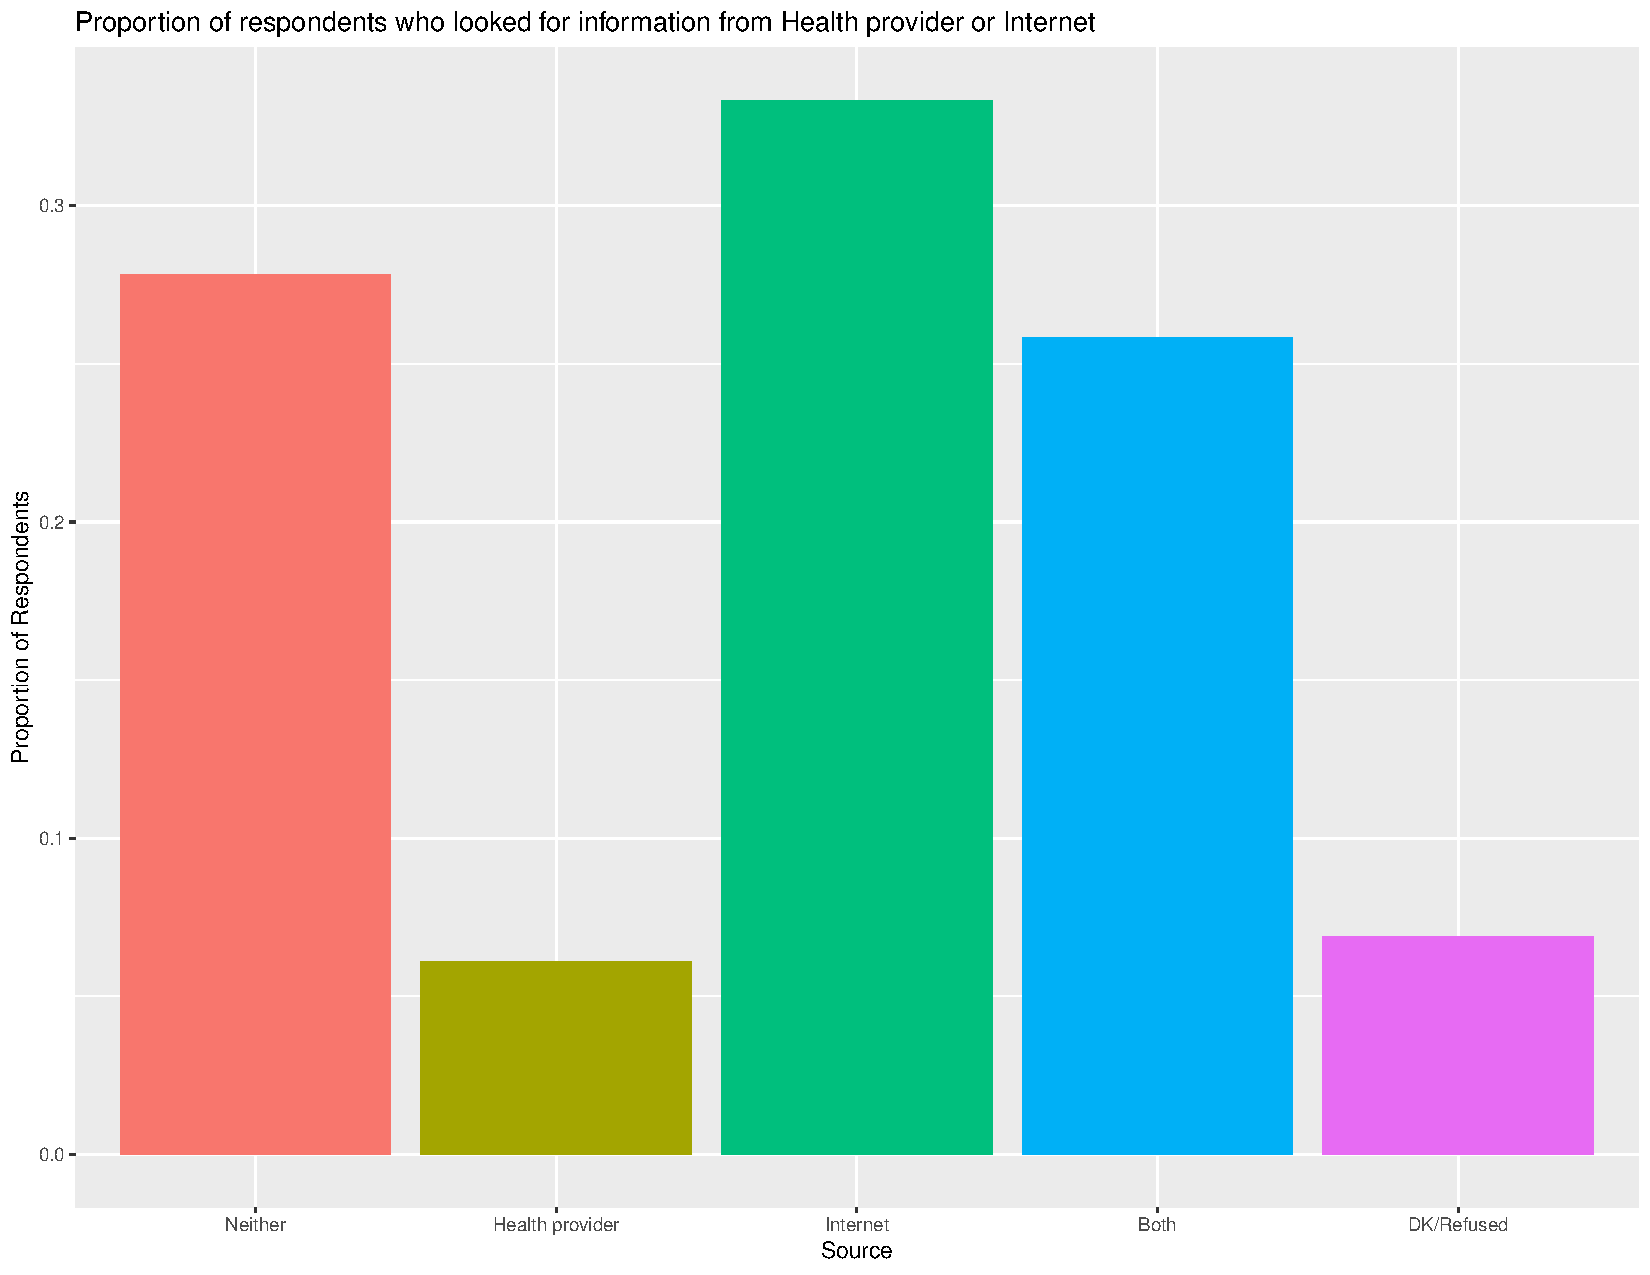
\includegraphics[width=.6\textwidth]{info_source.pdf}
  \caption{Far more respondents reported looking for information from Internet Sources compared with their healthcare provider}
\label{info_source}
\end{centering}
\end{figure}


\section{Query and Web Page Labeling}

\subsection{Overview of Labeling}
We used a hybrid human-computation method for labeling queries in the context of flu experience. We first define a labeling scheme for search queries. The scheme is designed to capture important differences in what the searcher is experiencing at the moment of executing a query|specifically flu-like experiences versus other experiences.
We used simple flu-related key words to isolate a subset of queries and web pages from each respondent's web history to be labeled by trained coders. Coders labeled each candidate query and page, then we joined those labels back to the survey data. This allows us to analyze the effects of different combinations of symptoms and demographics on flu search rates among respondents. This process reduced the number of queries and webpages to be labeled and resulted in high levels of intercoder agreement and reliability (see table ~\ref{intercoder_ag}).

Then, in order to generate an expansive list of flu-like queries for forecasting, we compute semantic distances between the positively-labeled set of queries and other queries executed in the Bing search engine. Based on this comparison, we retain all semantically-related queries from Bing and label them according to our scheme. This allows us to identify additional flu-like queries for our time-series forecasting models. We also computed intercoder agreement and reliability scores for this set (see table ~\ref{intercoder_bing}).

\subsection{Labeling Scheme}

In order to define a flu-related query or web page, we developed a labeling scheme to indicate whether each query or web page was likely related to a flu-like experience, versus experiences related to an array of non-flu infections (including the common cold), news, personal interest, and social trends. In our scheme, we differentiate flu-like experience queries from queries that are unrelated to a flu-like experience but nonetheless contain flu terms. For example, searches like `fever and cough 5 days', or `high fever body aches' would qualify as flu-like experience queries. By contrast, `flu pandemic', 'sore throat obama', or `1918 flu', would qualify as research-oriented and unrelated to a flu experience. Similarly, web pages containing information about flu-like symptoms (e.g. `fever' and `cough') would qualify as page visits related to flu-like experiences.

Among queries or pages that convey a flu-like experience, we further identify two forms: experiences of primary flu symptoms, in which one experiences the most common symptoms of flu  - fever and cough, and experiences of secondary symptoms, in which one experiences secondary (and less common) symptoms of flu (body aches, diarrhea, vomiting). Queries and web pages that appear consistent with a primary flu-like experience receive an `A1' label, and queries and pages consistent with secondary flu-like experiences receive a `B1' label. Queries and pages that appear related to flu but not deemed to be a flu-like experience (journalistic interest or research) receive an `A2' designation. `A1' labels capture the primary flu-like experience that we are interested in tracking and are the basis of our subsequent forecasting model. The remainder of the labels serve primarily as gut-checks to validate our data and results.

\subsection{Codebook: Descriptions of Labels}
\begin{itemize}
\item A1. Related to experienced ILI – symptoms of canonical flu definition (cough or fever [can be in combination with other symptoms), treatments for flu, generic flu searches/pages (as if from someone searching re how to diagnose or treat).

Examples: searches - “flu”, “cough”, “what to do if you have the flu”, “productive cough fever body aches”, “tamiflu information”; web pages - “Home Remedies for Flu Symptoms (WebMD)”; http://www.rxwiki.com/slideshow/surprising-facts-about-flu/chicken-soup-actually-helps.
Keep in mind that pages specifying diagnoses and remedy of canonical flu symptoms go in this category.

\item A2. Flu not in the context of experienced probable ILI – trends, prevention (including vaccination), policies, scientific background, etc.

Examples: Searches - ``flu epidemic'',``flu vaccine 23\% effective'', ``avian flu strain''; web pages - ``TABLE. Influenza Vaccines — United States, 2014–15 Influenza Season*,  Seasonal Influenza (Flu)  CDC”; ``Flu Activity \& Surveillance, Seasonal Influenza (Flu) , CDC''.

\item B1. Secondary flu symptoms (generic or as experienced) – sore throat, headache, body aches, fatigue, runny nose, stuffed up nose, vomiting, diarrhea.

Examples: searches - ``sore throat gargle salt water'', ``sore throat and breast pain'', ``3 year old runny nose only''; web pages – ``Is It a Cold or a Sinus Infection? Symptoms \& Treatments (WebMD)'', ``Sore Throat Home Remedies and Treatments''.

\item B2. Secondary flu symptoms not in the context of experienced probable ILI

Examples: searches – “tiger vomits on course”, “holiday vomit fest”, “pres. obama sore throat”

 \item C1. Other generic or experienced illness syndromes or symptoms – croup, pneumonia, stomach flu, ear infection, etc.

Examples: searches – ``can adults get croup'', ``whooping cough'', ``swollen toe'', ``cdc ebola''; web pages – \url{http://www.webmd.com/digestive-disorders/diarrhea-stomach-flu}, ``Middle ear mucus won't drain. Ear, Nose \& Throat Community - Support Group (WebMD)''

\item D. Unrelated to human illness

Examples: searches – “cat cough”, “frozen fever” “acdc rock or bust tour”, “marisa coughlan feet”, “saturday night fever soundtrack”; web pages – “Pflugerville, Texas - Wikipedia, the free encyclopedia”; “Influence and reception of Søren Kierkegaard - Wikipedia, the free encyclopedia”
\end{itemize}

\subsection{Labeling Queries and Pages from Respondent Browsing History}

Once we had a scheme for labeling queries and pages, we developed a strategy for locating candidate A1 queries from the survey data, given that each user in our panel executed anywhere from dozens to hundreds of queries during the survey period, and it would be inefficient to code every one of them.

To isolate a subsample of queries to label, we started with a simple set of keywords. Using the search history data from our panel, we located a subsample of queries that contained a set of predefined illness-related key words - including terms like: `sick', `flu', `fever', `cough', `ache', `vomiting', `sore throat'.

%Once the results of the survey were returned, we developed a strategy for locating candidate A1 queries from search histories, given that each user in our panel executed anywhere from dozens to hundreds of queries during the survey period, and it would be inefficient to code every one of them. To isolate a subsample of queries and pages to label, we start with a simple set of keywords. Using the search history data from our panel, we created a subsample of queries and web pages containing a set of predefined illness-related key words - including terms like: `sick', `flu', `fever', `cough', `ache', `vomiting', `sore throat'. We then tasked trained coders with labeling each of these queries according to our `A1' coding scheme. In this sample of queries, we found 21\% of respondents made an A1 query or page visit, and 14\% made an A2 query or page visit. These queries were used in our survey analysis. We joined the labeled queries back to the survey data over the 2014-2015 flu season. From there, we model the relationship between self-reported flu-like symptoms and whether a respondent executed an A1 query using our classic case-control design \citep{king_and_zeng_2001}.

For webpages, we selected a set of likely candidate base websites, including: cdc.gov, webmd.com, flu.gov, nih.gov, wikipedia.com, and mayoclinic. We then searched the clickstream for user access to flu related webpages within these domains using the ``flu'' keyword within the following search structure:

\begin{lstlisting}
where (page_url like '%cdc.gov%' and page_url like '%flu%' )
or (page_url like '%webmd.com%' and page_url like '%flu%')
or (page_url like '%flu.gov%')
or (page_url like '%nih.gov%' and page_url like '%flu%')
or (page_url like '%wiki%' and page_url like '%flu%')
or (page_url like '%mayoclinic%' and page_url like '%flu%')
\end{lstlisting}

We then tasked trained coders with labeling queries and pages according to our coding scheme (table ~\ref{intercoder_ag}. In this sample of queries and web pages, we found 21\% of respondents made an A1 query or page visit, 14\% made an A2 query or page visit, and 9\% made a B1 query or page visit. Intercoder reliability on this set was Kappa=.865 for search queries and Kappa=.796 for web pages (see table ~\ref{intercoder_ag}). In tables ~\ref{intercoder_queries} and ~\ref{intercoder_webpages}, we display confusion matrices displaying labeling choices from the two trained coders, and specific labels which created the most disagreement.

%This subsample provided a candidate set of queries and pages which could be labeled and fed into a word embedding model to uncover further relevant examples. %The primary distinction we sought to capture was whether a query was executed by a person experiencing ILI symptoms, rather than by a person searching for news, for research, or for an unrelated subject with a name containing flu terms. Like other studies, many search queries that contain flu-like terms are actually irrelevant to having the flu. For example, the terms ``frozen fever'', ``President Obama sore throat'' contain key terms that are not necessarily connected to an individual being sick with the flu. Our labeling process, relying on human coders and embedding algorithms, sifts through this language to root out this type of false positive. We describe this labeling process below. %Second, using these data we are able to statistically analyze the propensity to make flu-like queries based on demographic information, in order to extract individual-level insights and build an aggregate model. Coders sought to differentiate queries or page visits that someone would make if they were sick with the flu


\begin{table}[!htbp] \centering
  \caption{Intercoder Reliability - Survey Queries and Pages}
  \label{intercoder_ag}
\begin{tabular}{@{\extracolsep{5pt}} cccc}
\\[-1.8ex]\hline
\hline \\[-1.8ex]
 &  & Queries & Web Pages \\
\hline \\[-1.8ex]
 & N & $1422$ & $797$ \\
 & Agreement & $89\%$ & $85.7\%$ \\
 & Kappa & $0.865$ & $0.796$ \\
 & Z-score & $68.5$ & $36.8$ \\
 & p & $<0.01$ & $<0.01$ \\
 & Coders & $2$ & $2$ \\
\hline \\[-1.8ex]
\end{tabular}
\end{table}

\begin{table}[!htbp] \centering
  \caption{Intercoder Reliability of Panel Queries - Confusion Matrices}
  \label{intercoder_queries}
\begin{tabular}{@{\extracolsep{5pt}} ccccccc}
\\[-1.8ex]\hline
\hline \\[-1.8ex]
 &   Queries & &&&& \\
\hline \\[-1.8ex]
      &   A1 & A2 & B1 & B2 & C1 &  D \\
  A1 &   318 &  2 & 11 &  0 & 17 &  6\\
  A2    & 12 &120 &  0  & 0   &0 &  1\\
  B1     & 2  & 0 & 76 &  1 & 25 & 11\\
  B2    & 5  & 0 &  7& 257  & 5 & 10\\
  C1     &17  & 0 &  8  & 0& 283 &  6\\
  D     & 3 &  1 &  1 &  0 &  4& 213\\
\hline \\[-1.8ex]
\end{tabular}
\end{table}

\clearpage

\begin{table}[!htbp] \centering
  \caption{Intercoder Reliability of Panel Web Pages - Confusion Matrices}
  \label{intercoder_webpages}
\begin{tabular}{@{\extracolsep{5pt}} ccccccc}
\\[-1.8ex]\hline
\hline \\[-1.8ex]
 &   Web Pages & &&&& \\
\hline \\[-1.8ex]
      & A1 & A2 & B1 &B2 & C1 & D \\
A1 &  245&31&20& 0& 1& 0 \\
A2 &  18 & 263& 2& 0&28& 0 \\
B1 &  3& 1&25& 0& 1& 0 \\
B2 &  1& 0& 0& 0& 0& 0 \\
C1 &  1& 0& 3& 1 & 105& 1 \\
D  & 1& 0& 0& 0& 0&45 \\
\hline \\[-1.8ex]
\end{tabular}
\end{table}

The top 10 stemmed words from the respondent set of queries can be observed in table ~\ref{descript1}. The reader will note that these queries are not a random sample of queries from the web. Half of these queries came from users selected at the outset because they searched for a flu-related term, while the other half came from users who were selected because they matched the search volume of the first group within a narrow band but did not execute a flu-related query (see description in previous section). As a consequence of this matching process, illness-related words are more common in our sample than in a random draw of queries. We correct for this bias in our statistical models, described in the main text, and in following sections in the SI. In table ~\ref{descript2}, the top 10 stemmed words from all queries that matched the A1 criteria as judged by hired coders.

\begin{table}[!htbp] \centering
  \caption{Top Stemmed Words in All Queries (panel)}
  \label{descript1}
\begin{tabular}{@{\extracolsep{5pt}} cccc}
\\[-1.8ex]\hline
\hline \\[-1.8ex]
 & word & freq & proportion \\
\hline \\[-1.8ex]
  & flu & 257 & 0.0514 \\
 & vomit & 256 & 0.0512 \\
 & cough & 163 & 0.0326 \\
 & fever & 150 & 0.03 \\
 & sick & 99 & 0.0198 \\
 & diarrhea & 87 & 0.0174 \\
 & swollen & 84 & 0.0168 \\
 & sore & 83 & 0.0166 \\
 & girlfriend & 70 & 0.014 \\
 & throat & 70 & 0.014 \\
\hline \\[-1.8ex]
\end{tabular}
\end{table}

\begin{table}[!htbp] \centering
  \caption{Top Stemmed Words in A1 Queries (panel)}
  \label{descript2}
\begin{tabular}{@{\extracolsep{5pt}} cccc}
\\[-1.8ex]\hline
\hline \\[-1.8ex]
 & word & freq & proportion \\
\hline \\[-1.8ex]
 & cough & 101 & 0.12 \\
 & fever & 97 & 0.115 \\
 & ach & 14 & 0.017 \\
 & child & 14 & 0.017 \\
 & grade & 11 & 0.013 \\
 & infant & 11 & 0.013 \\
 & low & 11 & 0.013 \\
 & rash & 11 & 0.013 \\
 & sick & 10 & 0.012 \\
 & babi & 9 & 0.011 \\
\hline \\[-1.8ex]
\end{tabular}
\end{table}

\clearpage

\section{Query Data Geographic and Temporal Coverage}

Search query data provided in partnership with Bing cover years from 2012 to 2017 for all 50 states plus the District of Columbia. While we are unable to share overall rates of searches from Bing, we can share relative coverage rates for the states and years included. For the state rates, we counted the number of queries in each year, then normalized by population to generate a query rate per capita measure. We then subtracted the state average and divided by the standard error to generate a z-score. We did this separately for the overall query count, flu queries (queries that were flagged as likely related to flu based on our DOC2VEC expansion), and the A1 query count.

For the yearly rates, we calculated the average query count in each year, then subtracted the overall yearly mean and divided by the standard deviation to arrive at the z-score. The figures below show the calculated z-scores by state and year (see figures \ref{state_coverage} and \ref{year_coverage}).

\begin{figure}[!htbp]
\begin{centering}
   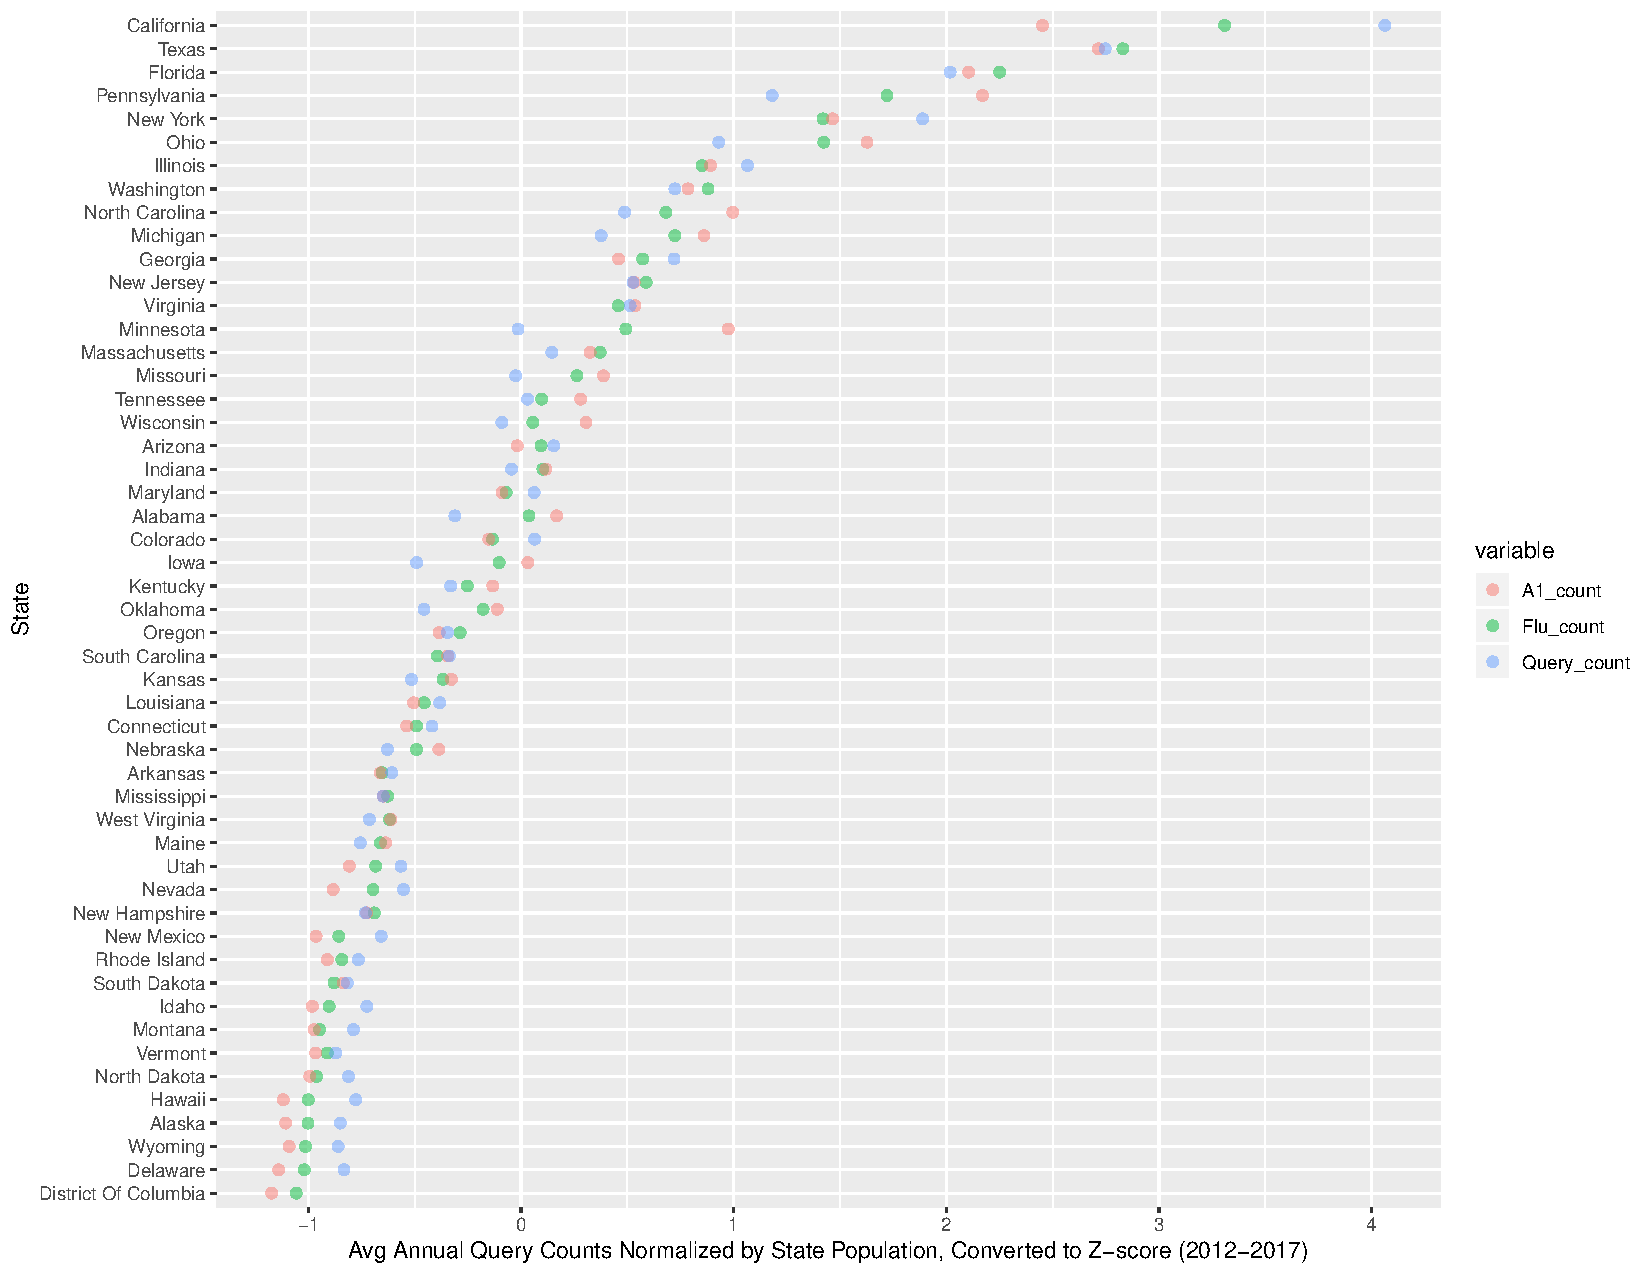
\includegraphics[width=1\textwidth]{state_coverage.pdf}
  \caption{State coverage of Bing queries 2012-2017}
\label{state_coverage}
\end{centering}
\end{figure}

\begin{figure}[!htbp]
\begin{centering}
   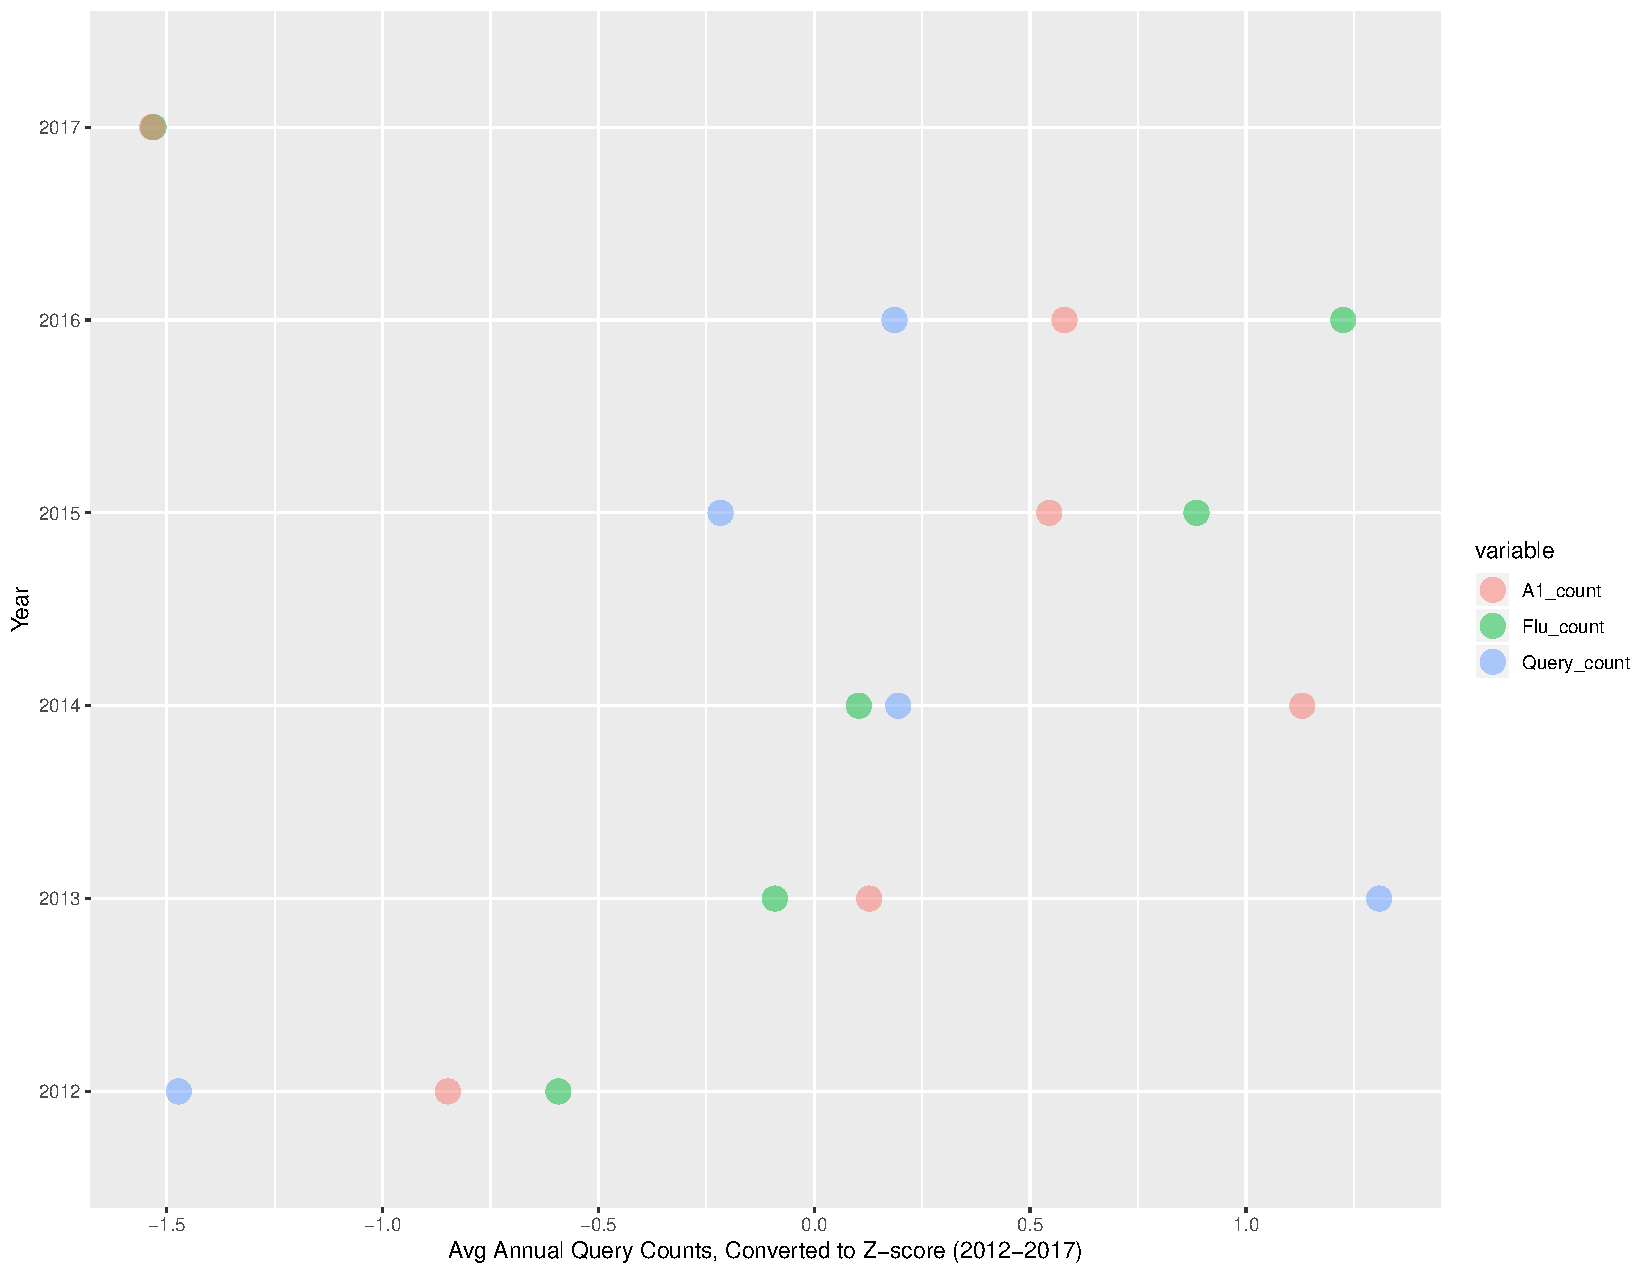
\includegraphics[width=1\textwidth]{yearly_coverage.pdf}
  \caption{Yearly coverage of Bing queries 2012-2017}
\label{year_coverage}
\end{centering}
\end{figure}

\subsection{Predicting Internet Behavior Based on Reported Symptoms}

This section provides some additional information on the reported symptoms in our panel and the relationship between these and flu.

\subsubsection{Descriptive Relationship}

The tables below give the co-occurrence of reported flu symptoms in the household (fever + cough), and queries coded for A1 and A2 in the respondent set of queries. Among respondents reporting flu-like symptoms in the household, roughly 28\% made A1 queries or visited relevant pages. Among respondents not reporting flu-like symptoms in the household, roughly 17\% made A1 queries or visited pages. In the tables, below we display basic descriptive cross-tabulations of the occurrence of flu symptoms with A1 search (ILI searches) and A2 searches (interest and research queries).

\begin{table}[!htbp]
\centering
  \caption{A1-coded Activities and Flu Symptoms in Household}
  \label{descript3}
\begin{tabular}{rrrr}
  \hline
    & not flu &  flu & \\
not A1 & 354 & 164 & 0.32\\
A1 & 72 & 64 & 0.47 \\
   \hline
   & 0.17 & 0.28 &  \\
   \hline
\end{tabular}
\end{table}

We construct the same table of A2 searches as table ~\ref{descript3} and compare it to flu symptoms on a subset of the data where respondents had not also executed an A1 query. We expect that since A2 activity is associated with interest or research, it will not be associated with flu symptoms. Here, we see that among respondents reporting flu-like symptoms, roughly 11\% made an A2 search, and among respondents not reporting flu-like symptoms, roughly 8\% made an A2 search.

\begin{table}[!htbp]
\centering
  \caption{A2 Searches and Flu Symptoms}
  \label{descript4}
\begin{tabular}{rrrr}
  \hline
    & not flu &  flu & \\
not A2 & 375 & 187 & 0.33 \\
A2 & 32 & 23 & 0.42 \\
   \hline
   & 0.08 & 0.11 & \\
   \hline
\end{tabular}
\end{table}

%The figure below visually depicts the correlations between stemmed query words and reported symptoms experienced by the respondent (Res.flu), in the home (House.Flu), by the spouse(Spouse.flu), and by a child (Child.flu). Darker blue indicates stronger positive correlations while darker red indicates stronger negative correlation.

%\begin{figure}[!htbp]
%\begin{centering}
%   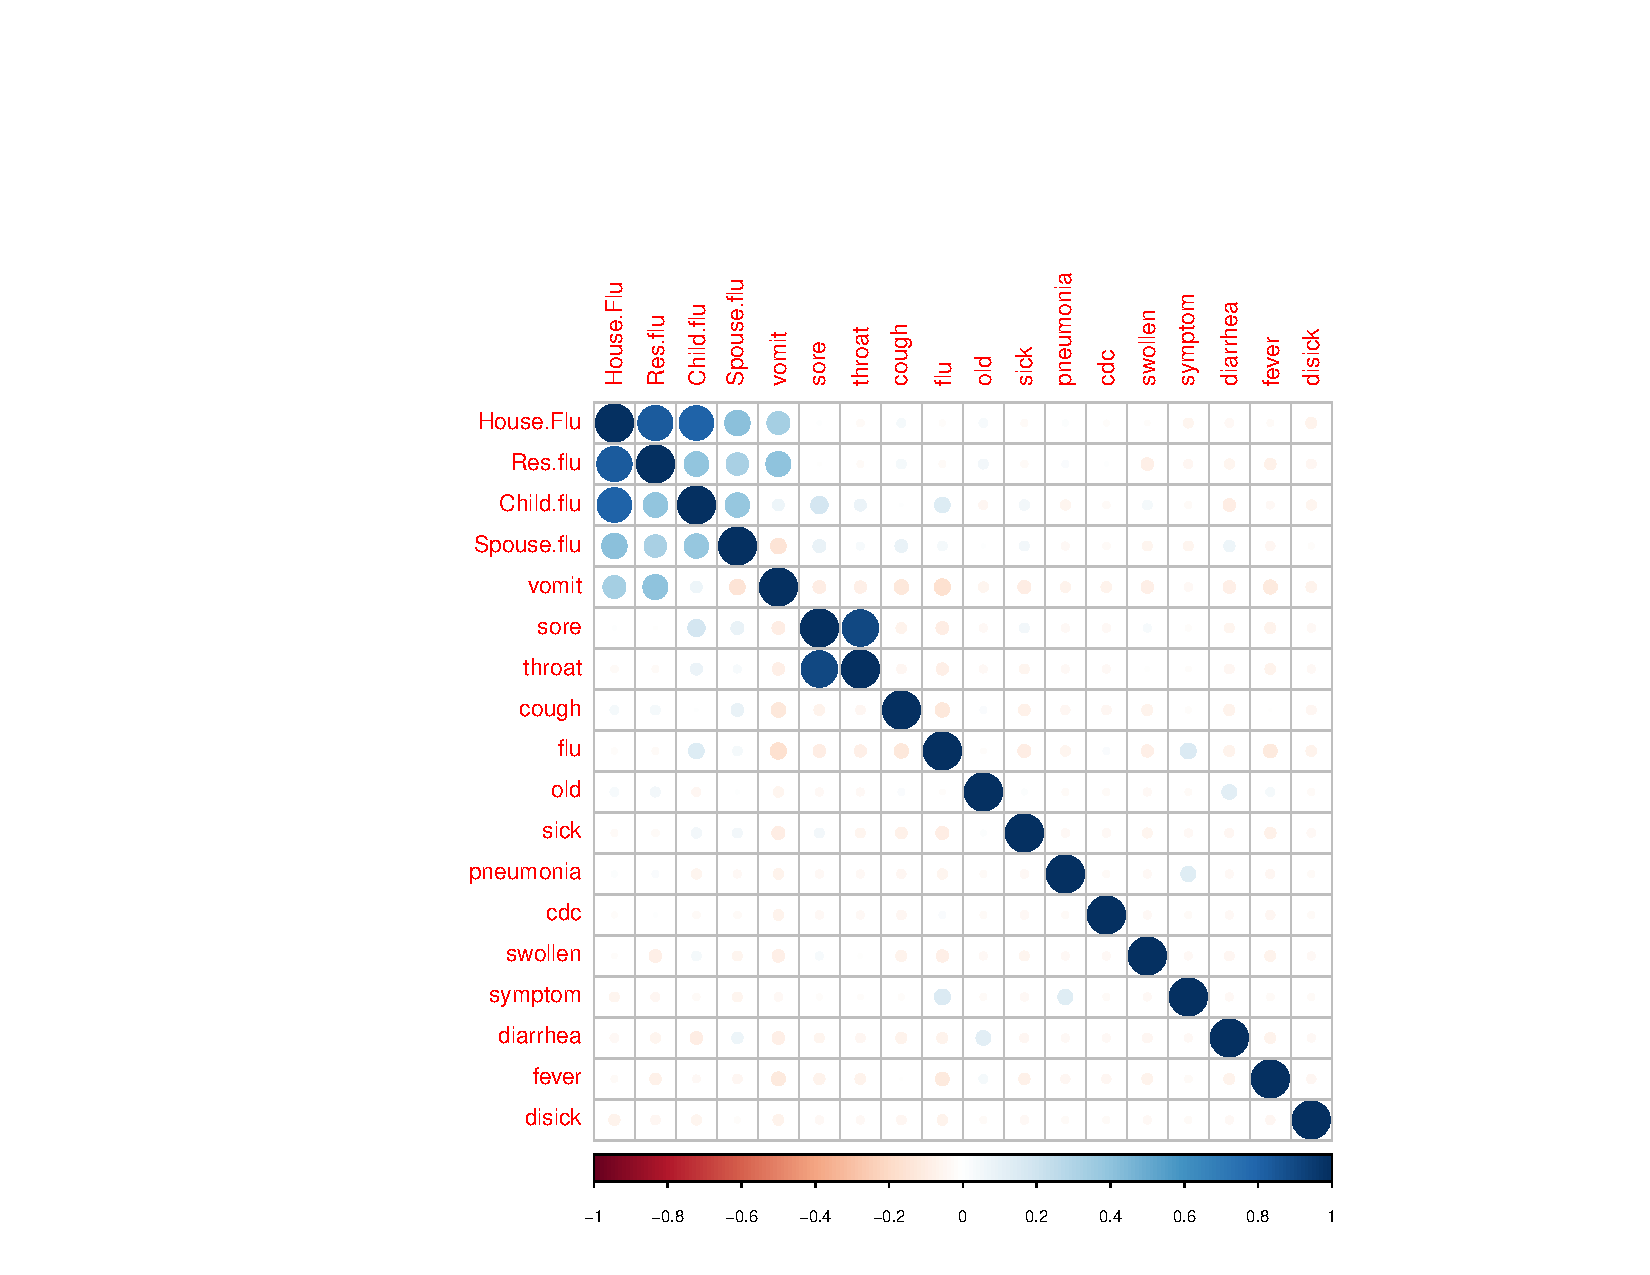
\includegraphics[width=1\textwidth]{fluterms_and_correlations}
%  \caption{Correlations of Flu and Flu Query terms}
%\label{corrs}
%\end{centering}
%\end{figure}

\subsubsection{Regression Model and Case-Control Design}

In order to infer the effect of flu-like experience on web activity, we regressed the occurrence of flu-related queries or page visits (A1) on self-reported flu symptoms and demographic characteristics. To infer the effect of the flu on A1 activity, we used a `classic' or `cumulative' case-control design. To do so, we first paired positive flu search cases with negative cases, then adjusted for sample differences between the data and the average rate of A1 flu searches from the Bing search engine (1.2e-5). This process allows us to reduce bias induced by the relatively rare occurrence of flu searches in the population. We estimate the search rate using a rare events logistic regression, where $Pr(Y_i=1|X_i) = \frac{1}{1+e^{ - (\beta_0 + X_i \beta ) }}$ . Where $\beta_0$ is a constant term, $X_i$ is a k-vector of covariates, and $\beta$ is a vector of coefficients.

We calculated the relative risk (RR) and risk difference (RD) of search activity given flu symptoms: $ RR = Pr(Y=1|X_1, \pi) / Pr(Y=1|X_0, \pi) $, $ RD = Pr(Y=1|X_1, \pi) - Pr(Y=1|X_0, \pi) $ \citep{king_and_zeng_2001}. Where $\pi_i$ is the incidence of A1 searches for user $i$, $X_1$ is a k-vector of covariates of a `treatment' group with flu symptoms and $X_0$ indicates a k-vector of covariates of a `control' group lacking flu symptoms. To control for the fact that the population's rate of A1 search differs from our sample, we substitute the constant term in the logistic model for a corrected term that matches the observed rate of flu search in the Bing search engine. This corrected term is calculated as: $B_0 - ln[ (\frac{1-\tau}{\tau}) (\frac{\bar{y}}{1-\bar{y}}) ]$, where $B_0$ is the original constant term, $\tau$ is the rate of A1 search in the population, and $\bar{y}$ is the rate of A1 search in the sample. The coefficients remain unbiased. Figure 1 in the main paper plots the expected values of $Y$, $Pr(Y=1|X, \tau)$, where household flu is present and absent.

% Take out this figure (in the main paper) and replace with the regression table

%\begin{figure}[!htbp]
%\begin{centering}
%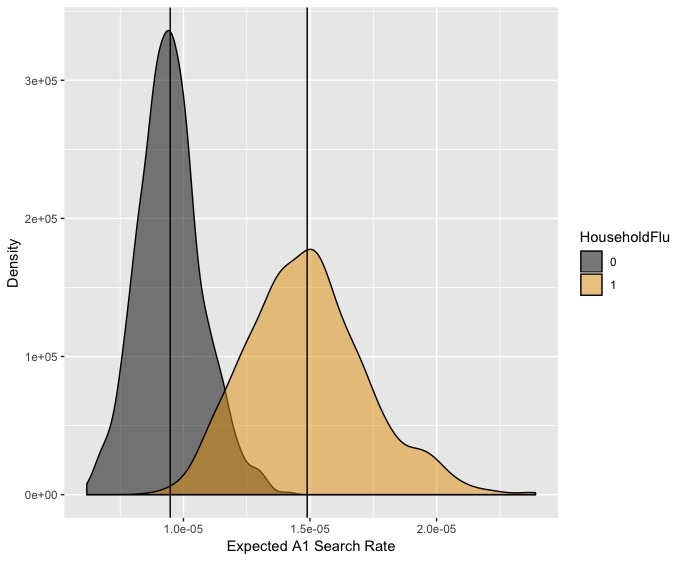
\includegraphics[width=1\textwidth]{Sim_QI_flu}
%  \caption{Expected search rates when flu is present/absent in household}
%\label{sim_qi_flu}
%\end{centering}
%\end{figure}

We find a heightened tendency to make both A1 and A2  searches/visits when there is an occurrence of flu symptoms in the household. In figure 1 in the main paper, the means of $ = Pr(Y=1|x_1, \pi)$ and $ Pr(Y=1|x_0, \pi) $ are shown with dark vertical lines. The estimated Risk Ratio (RR) is 1.57 (95\% CI = 1.05, 2.34), meaning that those with flu symptoms execute almost 60\% more A1 searches compared to those exhibiting no symptoms at all (see table ~\ref{table:coefficients_a1}). However, since the base rate is very low, this amounts to a Risk Difference (RD) of about 5.41e-06 (95\% CI = 5.57e-07, 1.09e-05), which relates to a very small change in the overall probability of an A1 search given flu symptoms. Nonetheless, the risk difference is statistically significant (p$<$.05).

 %Using these data in combination with the A1 query categorizations above,  %Table XX presents these regressions.

%We find that flu symptoms in the household are associated with a higher likelihood of a respondent making A1, A2, and B1 searches. Our findings suggest that reported flu-like symptoms are a precursor to making flu queries.

%These models suggest that when there is flu within the household (at least one person in the house has reported both a fever and a cough), the respondent is roughly 60\% more likely to make an A1 query/visit compared to when the household is asymptomatic (SI). In addition, we find that particular demographic variables - such as gender and age - are particularly predictive of flu-like queries in the presence of flu symptoms.

We also find that searches are noisy indicators for particular subgroups, specifically heavy searchers, women, and parents (see table ~\ref{table:coefficients_parents}). We find that A1 searches are correlated with having higher search volumes. People who search more will end up making A1 or A2 searches/visits by chance. Women tend to make more A1 and A2 searches/visits on average, and make many more `asymptomatic' searches compared to men (where a flu search occurs but no symptoms are reported). Among parents, we find that younger parents are more likely to make A1 searches/visits in the context of a child sick with flu and less likely to make A2 searches/visits. We tested to see if parents of young children are more likely to make A1 searches if their children have flu-like symptoms, but we found no statistically discernible effect.%\footnote{The way that respondents are asked about symptoms renders it difficult to discern exactly what combination of symptoms they were experiencing and when. As a result, a simple coding of flu as fever+cough contains a certain amount of measurement error. We cannot know with certainty if these canonical flu symptoms occurred together or separately.}

\begin{table}
\begin{center}
\begin{tabular}{l c c c c }
\hline
y = A1 Search & Model 1 & Model 2 & Model 3 & Model 4 \\
\hline
(Intercept)    & $-12.75^{***}$ & $-11.51^{***}$ & $-12.66^{***}$ & $-12.39^{***}$ \\
               & $(0.63)$       & $(1.12)$       & $(0.62)$       & $(0.67)$       \\
Household Flu  & $0.46^{*}$     &                &                &                \\
               & $(0.21)$       &                &                &                \\
Volume         & $0.15^{*}$     & $0.23$         & $0.15^{*}$     & $0.17^{*}$     \\
               & $(0.07)$       & $(0.12)$       & $(0.07)$       & $(0.08)$       \\
Female         & $0.72^{**}$    & $0.42$         & $0.74^{***}$   & $0.65^{**}$    \\
               & $(0.22)$       & $(0.37)$       & $(0.22)$       & $(0.24)$       \\
Parent         & $0.33$         &                & $0.44^{*}$     &                \\
               & $(0.22)$       &                & $(0.21)$       &                \\
Age            & $-0.05$        & $-0.42^{*}$    & $-0.06$        & $-0.08$        \\
               & $(0.07)$       & $(0.17)$       & $(0.07)$       & $(0.08)$       \\
Child Flu         &                & $0.60$         &                &                \\
               &                & $(0.33)$       &                &                \\
Respondent Flu          &                &                & $0.31$         &                \\
               &                &                & $(0.22)$       &                \\
Spouse Flu          &                &                &                & $0.06$         \\
               &                &                &                & $(0.29)$       \\
\hline
AIC            & 645.40         & 233.19         & 648.12         & 523.02         \\
BIC            & 672.21         & 249.75         & 674.93         & 544.17         \\
Log Likelihood & -316.70        & -111.59        & -318.06        & -256.51        \\
Deviance       & 633.40         & 223.19         & 636.12         & 513.02         \\
Num. obs.      & 644            & 203            & 644            & 507            \\
\hline
\multicolumn{5}{l}{\scriptsize{$^{***}p<0.001$, $^{**}p<0.01$, $^*p<0.05$}}
\end{tabular}
\caption{Rare events models of A1 flu activity online}
\label{table:coefficients_a1}
\end{center}
\end{table}

\clearpage
\newpage

We next re-run our analyses with A2 searches as the outcome variable of interest on a subset of the data where respondents had not executed an A1 query but had executed an A2 query. This serves as a validation check to determine whether A2 or interest-oriented searches are indeed false positive searches. We find no detectable effect of flu symptoms of any household member on the occurrence of A2 research or interest-oriented searches in this subset of the data (see table ~\ref{table:coefficients_a2}).

\begin{table}
\begin{center}
\begin{tabular}{l c c c c }
\hline
y=A2 & Model 1 & Model 2 & Model 3 & Model 4 \\
\hline
(Intercept)    & $-13.38^{***}$ & $-14.55^{***}$ & $-13.23^{***}$ & $-12.56^{***}$ \\
               & $(0.95)$       & $(1.93)$       & $(0.94)$       & $(0.97)$       \\
Household flu  & $0.41$         &                &                &                \\
               & $(0.31)$       &                &                &                \\
Search volume         & $0.19$         & $0.05$         & $0.19$         & $0.08$         \\
               & $(0.10)$       & $(0.19)$       & $(0.10)$       & $(0.11)$       \\
Female         & $0.50$         & $0.53$         & $0.52$         & $0.43$         \\
               & $(0.31)$       & $(0.60)$       & $(0.31)$       & $(0.34)$       \\
Parent         & $-0.10$        &                & $0.00$         &                \\
               & $(0.33)$       &                & $(0.32)$       &                \\
Age            & $0.11$         & $0.48$         & $0.10$         & $0.10$         \\
               & $(0.10)$       & $(0.28)$       & $(0.10)$       & $(0.12)$       \\
Child flu         &                & $1.01$         &                &                \\
               &                & $(0.55)$       &                &                \\
Respondent flu          &                &                & $0.08$         &                \\
               &                &                & $(0.33)$       &                \\
Spouse flu          &                &                &                & $0.36$         \\
               &                &                &                & $(0.39)$       \\
\hline
AIC            & 373.02         & 118.71         & 374.71         & 304.95         \\
BIC            & 399.47         & 134.97         & 401.16         & 325.78         \\
Log Likelihood & -180.51        & -54.35         & -181.35        & -147.48        \\
Deviance       & 361.02         & 108.71         & 362.71         & 294.95         \\
Num. obs.      & 607            & 191            & 607            & 476            \\
\hline
\multicolumn{5}{l}{\scriptsize{$^{***}p<0.001$, $^{**}p<0.01$, $^*p<0.05$}}
\end{tabular}
\caption{Rare events models of A2 activity. The sample is a subset of the data in which respondents did not make a concurrent A1 search.}
\label{table:coefficients_a2}
\end{center}
\end{table}

\subsection{Demographic Groups and Queries}

We find that flu-related searches are more likely among particular subgroups, specifically heavy searchers, women, and parents. A1 searches are correlated with having higher search volumes, and people who search more will end up making A1 or A2 searches/visits by chance. Women tend to make more A1 and A2 searches/visits on average, and make many more `asymptomatic' searches compared to men (where a flu search occurs but no symptoms are reported).

Among parents, younger parents are more likely to make A1 searches/visits in the context of a child sick with flu and less likely to make A2 searches/visits than older parents. To estimate these effects, we isolated the data to respondents who claimed to be the primary users of their devices (coded as those who claim to use their devices 80\% or more of the time relative to spouses and others in the household). We did this to ensure that search activity was limited to the parent and not the child, although the effects are substantial and significant in the broader sample as well. We found that fathers and mothers have different behaviors in reaction to perceived child illness. We find fathers to be much more likely to make A1 searches when their children have an ILI, whereas mothers tend to have a high baseline tendency to make such searches regardless of child illness (see figure ~\ref{mothers_a1}). Fathers more than 8 times as many A1 searches when their children exhibit ILI symptoms compared to when they are symptom-free (RR = 8.75, 95\% CI = 2.21, 42.36), which amounts to a risk difference of RD=1.95e-05 (95\% CI = 5.16-06, 4.53e-05) (see figure ~\ref{fathers_a1}). By contrast, we find no such moderating effects for A2 queries - mothers and fathers tend not to exhibit statistically significant differences in A2 search behavior when their children are ill with ILI.

\begin{figure}[!htbp]
\begin{centering}
   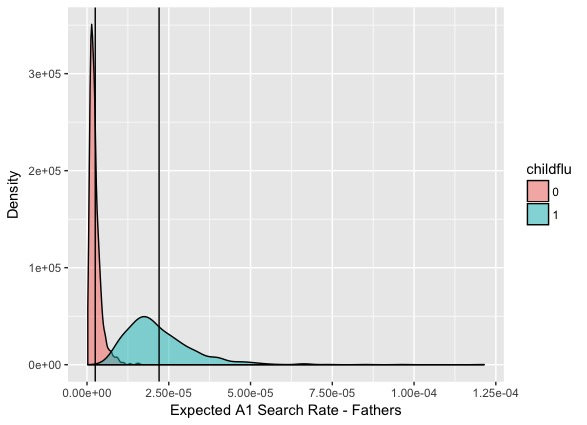
\includegraphics[width=.6\textwidth]{Exp_A1_Fathers}
  \caption{Father A1 searches when child flu present and absent}
\label{fathers_a1}
\end{centering}
\end{figure}

\begin{figure}[!htbp]
\begin{centering}
   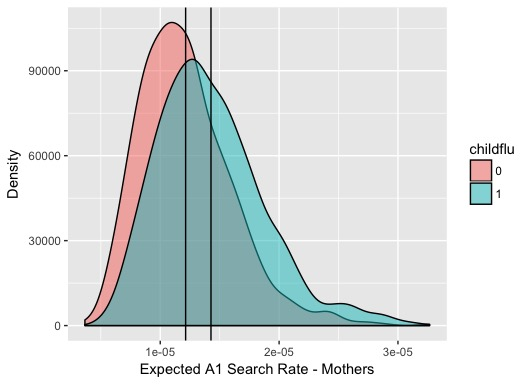
\includegraphics[width=.6\textwidth]{Exp_A1_Mothers}
  \caption{Mother A1 searches when child flu present and absent}
\label{mothers_a1}
\end{centering}
\end{figure}

\begin{table}
\begin{center}
\begin{tabular}{l c c }
\hline
 & y = A1 Search & y = A2 Search (subset) \\
\hline
(Intercept)              & $-12.97^{***}$ & $-14.55^{***}$ \\
                         & $(1.41)$       & $(1.97)$       \\
Child flu                   & $2.26^{**}$    & $1.12$         \\
                         & $(0.77)$       & $(0.98)$       \\
Parent gender - Moms        & $1.73^{*}$     & $0.73$         \\
                         & $(0.71)$       & $(0.91)$       \\
Volume                   & $0.39^{**}$    & $0.06$         \\
                         & $(0.14)$       & $(0.20)$       \\
Age                      & $-0.56^{**}$   & $0.45$         \\
                         & $(0.20)$       & $(0.28)$       \\
Child flu * Parent gender - Moms & $-2.10^{*}$    & $-0.34$        \\
                         & $(0.88)$       & $(1.17)$       \\
\hline
AIC                      & 191.93         & 117.04         \\
BIC                      & 211.09         & 135.82         \\
Log Likelihood           & -89.97         & -52.52         \\
Deviance                 & 179.93         & 105.04         \\
Num. obs.                & 180            & 169            \\
\hline
\multicolumn{3}{l}{\scriptsize{$^{***}p<0.001$, $^{**}p<0.01$, $^*p<0.05$}}
\end{tabular}
\caption{Rare events models of A1 flu activity online}
\label{table:coefficients_parents}
\end{center}
\end{table}

Differences in A1 search rates among self-identified racial categories were not significant in our sample. Similarly, differences in A1 search rates among self-reported education levels were not significant. See table ~\ref{table:race_coefficients} for these results. However, existing surveys using nationally-representative samples suggest that differences Internet usage exist with regard to age, income, education, and other demographic characteristics (\url{http://www.pewinternet.org/fact-sheet/internet-broadband/}). We control for demographic differences along these lines in our forecasting models.

\begin{table}
\begin{center}
\begin{tabular}{l c }
\hline
 & Model 1 \\
\hline
(Intercept)            & $-11.42^{***}$ \\
                       & $(0.25)$       \\
Household Flu          & $0.64^{**}$    \\
                       & $(0.20)$       \\
Education - No HS         & $-1.50$        \\
                       & $(1.06)$       \\
Education - Some College  & $-0.17$        \\
                       & $(0.31)$       \\
Education - Assoc. Degree & $0.23$         \\
                       & $(0.37)$       \\
Education - Bach. Degree  & $-0.21$        \\
                       & $(0.30)$       \\
Education - Grad. Degree  & $-0.22$        \\
                       & $(0.35)$       \\
Race - Black              & $-0.07$        \\
                       & $(0.36)$       \\
Race - Native             & $-0.47$        \\
                       & $(1.11)$       \\
Race - Asian-Pacific      & $0.06$         \\
                       & $(0.39)$       \\
Race - Hispanic           & $-0.06$        \\
                       & $(0.44)$       \\
Race - Other              & $10.85$        \\
                       & $(637.46)$     \\
Race - DK                 & $27.34$        \\
                       & $(819.58)$     \\
\hline
AIC                    & 674.68         \\
BIC                    & 732.96         \\
Log Likelihood         & -324.34        \\
Deviance               & 648.68         \\
Num. obs.              & 654            \\
\hline
\multicolumn{2}{l}{\scriptsize{$^{***}p<0.001$, $^{**}p<0.01$, $^*p<0.05$}}
\end{tabular}
\caption{Statistical models}
\label{table:race_coefficients}
\end{center}
\end{table}

\subsection{Classifying Flu Cases}

While household ILI symptoms may produce A1 activity by an individual, the question remains whether A1 searches and visits provide reliable predictive signals to classify an individual as having ILI symptoms. In order to further validate our coding methodology in a predictive task, we use a machine learning approach to assess the predictive power of the search queries for classifying cases as flu or not. We build basic classification models to classify reported flu occurrence at the household level and the respondent level. In each model, we set aside 30\% of the data for validation, leaving the remaining 70\% to build and test our models. We use a random forests algorithm to classify each respondent as having an ILI experience or not. We then plot the relative contribution of each variable to the model by examining the increase in accuracy from that variable relative to a random permutation of itself \citet{breiman_2001random}. We calculate these importance scores for each variable then scale them by dividing by the highest score and multiplying by 100 \citep{kuhn_2008, kuhn_and_johnson_2013} (see figure ~\ref{house_rf}). Random forest models were parameterized using using 25 bootstrap replications on the training data (all selected mtry=2 for the random forests).

\begin{table}[!htbp]
\centering
  \caption{Confusion Matrix: Household Flu (validation set)}
  \label{classif1}
\begin{tabular}{rrr}
  \hline
    & Reference &   \\
Prediction    &      $\neg{flu}$  &  flu\\
                $\neg{flu}$ & 49 (.47)  & 22 (.21)  \\
                          flu & 14 (13)  &  20 (.19) \\
   \hline
   Sensitivity &   &  0.476 \\
   Specificity & 0.778  &   \\
   \hline
\end{tabular}
\end{table}


Household ILI is defined as when a respondent reports one or more of the members of the household have fever and cough. Approximately 40\% of respondents reported at least one case of flu in the household. The rate of reported ILI was nearly identical in the training and validation sets - about 41\% (n=249) and 40\%(n=105), respectively. The random forest model yielded 66.1\% accuracy on the training set, and 65.7\% accuracy on the validation set (see table ~\ref{classif1}). The top five predictors of ILI occurrence were age, search volume, being a parent, religion, and education. `A1' queries were the most predictive of all the coded query types, ranking sixth overall in variable importance measures. Figure 2 displays the variable importance scores from the Household flu model. As above, these scores give the increase in model accuracy relative to a random permutation of each variable.

The household ILI model is able to correctly exclude nearly 80\% of non-flu cases in the data (see sensitivity in table ~\ref{classif1}). It was more difficult for the model to correctly include flu cases, creating a higher false positive rate than false negative rate. The true positive rate (sensitivity) was roughly 47.6\%.

\begin{figure}[!htbp]
\begin{centering}
   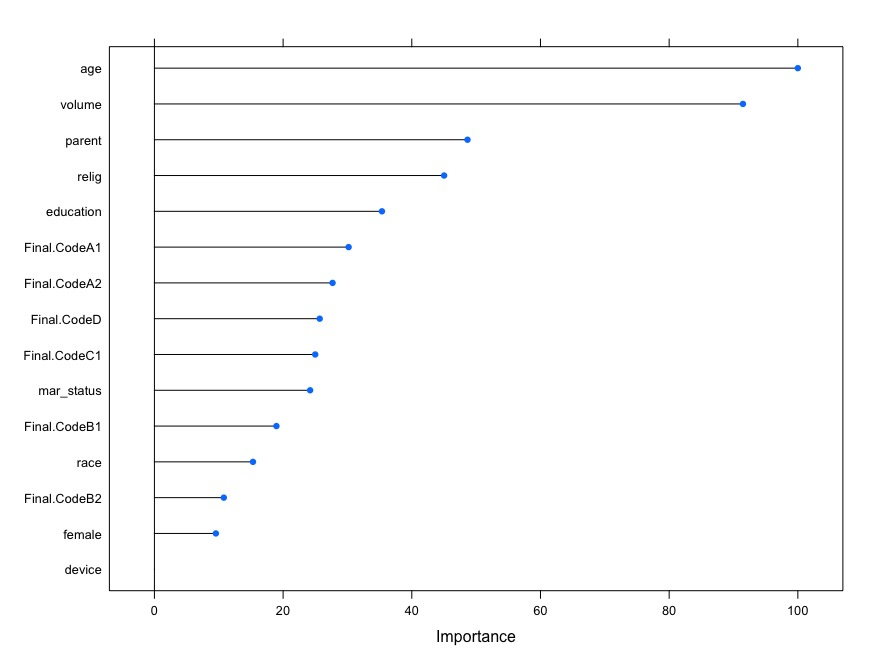
\includegraphics[width=.7\textwidth]{house_flu_rf_varimp}
  \caption{Household Flu Model Variable Importance}
\label{house_rf}
\end{centering}
\end{figure}

\clearpage

\subsection{Robustness Checks: Alternative Panel Models}

One potential criticism of our panel analysis is the choice to label a flu-like experience as when an individual reports having both a fever and cough, rather than fever and cough or fever and sore throat. We chose the former operationalization of flu to avoid ruling out (false positive) cases where a respondent reported a sore throat in the context of a separate (non-ILI) illness. Nonetheless, we re-analyzed our panel data with a flu-like experience coded as when a respondent reports fever and cough \emph{or} fever and sore throat.

\begin{table}[h!]
\begin{center}
\begin{tabular}{l c c c c }
\hline
y = A1 Search & Model 1 & Model 2 & Model 3 & Model 4 \\
\hline
(Intercept)    & $-12.73^{***}$ & $-11.38^{***}$ & $-12.65^{***}$ & $-12.27^{***}$ \\
               & $(0.61)$       & $(1.10)$       & $(0.61)$       & $(0.66)$       \\
Household Flu  & $0.45^{*}$     &                &                &                \\
               & $(0.21)$       &                &                &                \\
Volume         & $0.18^{**}$    & $0.24^{*}$     & $0.18^{**}$    & $0.18^{*}$     \\
               & $(0.07)$       & $(0.12)$       & $(0.07)$       & $(0.08)$       \\
Female         & $0.69^{**}$    & $0.48$         & $0.70^{***}$   & $0.65^{**}$    \\
               & $(0.21)$       & $(0.37)$       & $(0.21)$       & $(0.24)$       \\
Parent         & $0.25$         &                & $0.35$         &                \\
               & $(0.21)$       &                & $(0.20)$       &                \\
Age            & $-0.09$        & $-0.48^{**}$   & $-0.09$        & $-0.12$        \\
               & $(0.07)$       & $(0.17)$       & $(0.07)$       & $(0.08)$       \\
Child flu         &                & $0.57$         &                &                \\
               &                & $(0.33)$       &                &                \\
Respondent flu          &                &                & $0.33$         &                \\
               &                &                & $(0.21)$       &                \\
Spouse flu          &                &                &                & $-0.03$        \\
               &                &                &                & $(0.28)$       \\
\hline
AIC            & 668.37         & 234.20         & 670.71         & 530.73         \\
BIC            & 695.18         & 250.77         & 697.51         & 551.87         \\
Log Likelihood & -328.18        & -112.10        & -329.35        & -260.36        \\
Deviance       & 656.37         & 224.20         & 658.71         & 520.73         \\
Num. obs.      & 644            & 203            & 644            & 507            \\
\hline
\multicolumn{5}{l}{\scriptsize{$^{***}p<0.001$, $^{**}p<0.01$, $^*p<0.05$}}
\end{tabular}
\caption{Statistical models}
\label{table:coefficients}
\end{center}
\end{table}

The results are similar and consistent with our findings above - rates of flu search are variable across different types of users but are associated with flu symptoms. When flu is reported at the household level, RR = 1.55 (95\% CI = 1.042, 2.32), which amounts to a risk difference of RD=5.22e-06 (95\% CI = 4.52e-07 1.04e-05), and these differences are statistically significant.

When reexamining the differential effects of mothers and fathers using this alternative measure of flu, when find that fathers have a greater likelihood of flu search in the presence of child flu-like illness compared to mothers|similar to the results presented earlier. In the figure below, we plot this effect. For fathers, we find RR = 7.61 (95\% CI = 1.97, 36.76) and RD = 1.60e-5 (95\% CI = 3.91e-06 3.70e-05). These effects are slightly milder than those observed above, but we also see somewhat wider variation of the effect under this alternative measurement regime. %We suspect this is due to a high prevalence of sore throat occurring in non-flu illnesses.

\begin{figure}[!htbp]
\begin{centering}
   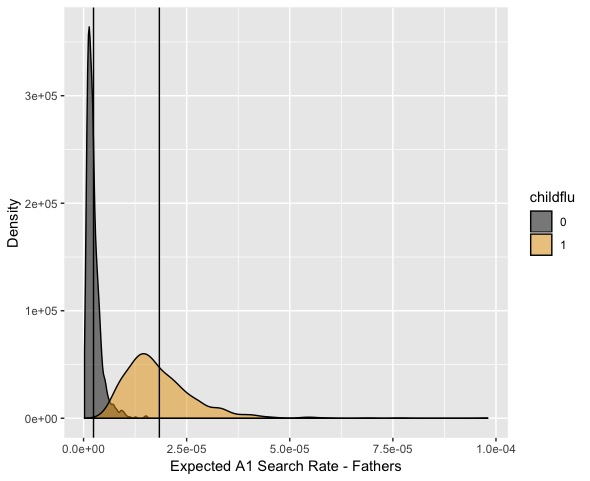
\includegraphics[width=.7\textwidth]{alternative_fathers}
  \caption{Effect of child flu under alternative flu measure - fathers}
\label{alt_fathers}
\end{centering}
\end{figure}


\subsection{Takeaways from Panel Analysis}

We find evidence to support the claim that search behavior is related to ILI in the household, but also to search volume, age, and gender. Our analysis suggests that a number of different patterns are important. First, not all queries containing the word `flu' are predictive of ILI experiences. Second, the propensity to conduct searches given ILI experiences (either in the respondent, the household, or in children), is not evenly distributed across demographic groups - as illustrated by the finding that the propensity to search for flu information is correlated with gender, parenthood, and age. This finding poses a challenge for forecasting, because the spread of the flu is also likely to be correlated with demographic features. This analysis raises further questions about methods which do not account for variability across demographic groups when forecasting ILI with web search data.

\section*{ILI Tracking Model}

We next describe the multi-step process of building a flu-tracking model using the insights from the case-control model just described. To do so, we first use word-embedding techniques to generate an expanded list of `A1' search queries based on similar searches in the Bing search engine. We do this since the queries in our relatively small survey are unlikely to capture all the possible queries meeting our our `A1' criteria. Then, we collect a sample of search queries from the Bing search engine and geo-locate them to their origin zip codes. We append census information at the zip code level and use multilevel regression with poststratification to generate a smoothed and re-weighted estimate of observed `A1' activity over the flu season. This estimate is adjusted for demographic features at the zip code level based on census information. This `A1' smoothed estimate is used as the primary predictor of CDC flu prevalance in an ARIMA time-series model.

\subsection*{Selecting and Labeling Additional Bing Queries}

Using the labeled subsample of queries matching predefined key words from our panel, we then used an embedding method called 'DOC2VEC' \citep{le_and_mikolov_2014} to find queries that are closely related to unseen A1 queries. This allowed us to create an expanded set of likely flu-related queries from the Bing engine for purposes of building our forecasting model. The DOC2VEC method creates document representations based on word embeddings learned from a corpus of text. These word embeddings capture deeper co-occurrence relations that are useful when trying to retrieve similar documents. In this case, our goal was to capture deep co-occurrences with A1 queries from our panel and queries executed on the Bing search engine. We trained a DOC2VEC model on our corpus of A1 labeled queries from our panel containing the word ``flu" or ``influenza". Based on this model, we retrieved the $10$-nearest neighbors using the Euclidean distance on this representation. We discovered that our approach often captured similarities based on misspelled queries, for example "caugh" and "cough". This information would be lost if instead we trained the word representations on a standard source like Wikipedia.

Based on our DOC2VEC expanded sample of queries, we asked coders to apply the same query labeling scheme as described above. The results of this coding can be seen in table ~\ref{intercoder_bing}, and in a confusion matrix of coding choices in table ~\ref{intercoder_bing_confusion}. Coder agreement in this expanded set was lower than in the respondent set of queries, likely due to somewhat greater heterogeneity of queries and possibly confusing misspellings. In table ~\ref{bing_all_stemmed} and table ~\ref{bing_a1_stemmed} we display the top 10 stemmed queries among all expanded queries and in all expanded queries that were coded as A1, respectively.

\begin{table}[!htbp] \centering
  \caption{Intercoder Reliability - Expanded Queries from Bing}
  \label{intercoder_bing}
\begin{tabular}{@{\extracolsep{5pt}} ccc}
\\[-1.8ex]\hline
\hline \\[-1.8ex]
 &  & Queries  \\
\hline \\[-1.8ex]
 & N & $1869$  \\
 & Agreement & $76\%$  \\
 & Kappa & $0.57$  \\
 & Z-score & $33.2$ \\
 & p & $<0.01$  \\
 & Coders & $2$ \\
\hline \\[-1.8ex]
\end{tabular}
\end{table}

\begin{table}[!htbp] \centering
  \caption{Intercoder Reliability of Expanded Bing Queries - Confusion Matrices}
  \label{intercoder_bing_confusion}
\begin{tabular}{@{\extracolsep{5pt}} ccccccc}
\\[-1.8ex]\hline
\hline \\[-1.8ex]
 &   Web Pages & &&&& \\
\hline \\[-1.8ex]
      & A1 & A2 & B1 &B2 & C1 & D \\
A1 &   824&  2&   0&  0&   5&   1 \\
A2 &   348 & 501& 0&  0&   0  & 7\\
B1 &    4&   0 &  1&  0&   0&   0 \\
B2 &    4&   2&   0&  0&  0&    0 \\
C1 &   61&   6&    0&  0 & 26&  7 \\
D  &   7&    3&    0&  0&  1&   59 \\
\hline \\[-1.8ex]
\end{tabular}
\end{table}

\begin{table}[!htbp] \centering
  \caption{Top Stemmed Words in All Queries (Bing)}
  \label{bing_all_stemmed}
\begin{tabular}{@{\extracolsep{5pt}} cccc}
\\[-1.8ex]\hline
\hline \\[-1.8ex]
 & word & freq & proportion \\
\hline \\[-1.8ex]
1 & flu & $1,425$ & $0.224$ \\
2 & shot & $292$ & $0.046$ \\
3 & influenza & $283$ & $0.045$ \\
4 & vaccin & $182$ & $0.029$ \\
5 & symptom & $121$ & $0.019$ \\
6 & stomach & $93$ & $0.015$ \\
7 & cough & $89$ & $0.014$ \\
8 & fever & $73$ & $0.011$ \\
9 & period & $58$ & $0.009$ \\
10 & incub & $47$ & $0.007$ \\
\hline \\[-1.8ex]
\end{tabular}
\end{table}

\begin{table}[!htbp] \centering
  \caption{Top Stemmed Words in A1 Queries (Bing)}
  \label{bing_a1_stemmed}
\begin{tabular}{@{\extracolsep{5pt}} cccc}
\\[-1.8ex]\hline
\hline \\[-1.8ex]
 & word & freq & proportion \\
\hline \\[-1.8ex]
1 & flu & $554$ & $0.223$ \\
2 & cough & $132$ & $0.053$ \\
3 & fever & $93$ & $0.037$ \\
4 & remedi & $63$ & $0.025$ \\
5 & symptom & $63$ & $0.025$ \\
6 & cold & $57$ & $0.023$ \\
7 & influenza & $33$ & $0.013$ \\
8 & headach & $28$ & $0.011$ \\
9 & medicin & $28$ & $0.011$ \\
10 & medic & $27$ & $0.011$ \\
\hline \\[-1.8ex]
\end{tabular}
\end{table}

\clearpage


\subsection{Accounting for Demographics: Query Smoothing and Re-weighting}

If flu search is unevenly spread across subgroups in the population, it then becomes important to control for flu search rates stemming from distinct demographic groups when forecasting flu prevalence within that population. In order to make estimates of flu based on search data, we generate a demographically-weighted estimate of A1 flu search rates over time based on Bing search data. This time-series serves as a demographically-sensitive indicator of underlying rates of flu.

To do so, we collected a long time-series of anonymized web search data from the Bing search engine for a period spanning from early 2011 to late 2016. We geolocated every query to a zip code and classified it as an A1 flu query based on the data coded from the survey panel labeled with the DOC2VEC and human-coder ensemble method. We linked each query to demographic data from the American Community Survey according to its origin zip code.

Based on the demographic information at the zip code level, we used a method called `multilevel regression with post-stratification' (MRP) to smooth (noise-reduce) and re-weight (reduce bias) against demographic variance in search behaviors \citep{gelman_and_little_1997, park_gelman_bafumi_2004}. This approach is typically used in survey research to control for sampling bias across demographic groups. We use it to 1) make estimates of flu search behavior across all zip codes at a granular time-scale, and 2) re-weight those estimates by demographic strata shown to be important in our individual-level model.

The MRP method leverages a property of multilevel modeling, ``shrinkage'', to reduce variance of estimates for units with few observations. In our case, this technique removes noise in flu search rates from less-common geographic areas by bringing them closer to the grand mean of all units. Then, we re-weight all estimates by the prevalence of units with similar demographic characteristics in the census data, we arrive at a population-level estimate of A1 flu-like search propensity.

The MRP model is constructed as follows:

$Pr(y_i = 1) = logit^{-1}( \beta_0  + \beta_{[it]}^{Income}
+ \alpha_{j[it]}^{State}
+ \alpha_{j[it]}^{Education}
+ \alpha_{j[it]}^{Age} \\
+ \alpha_{j[it]}^{Child-per-House}
+ \alpha_{j[it]}^{Education*Age} $
\\

Effect are assumed to be drawn from a normal distribution and estimated variance. \\

%\noindent
%$\alpha_j^{State} \sim  N (0, \sigma_{State}^2), \forall h = 1, ...., 52  $ \\
%$\alpha_k^{Education} \sim  N (0, \sigma_{Education}^2), \forall q = 1, ..., 4  $ %\\
%$\alpha_p^{Age} \sim  N (0, \sigma_{Age}^2), for l = 1, ..., 4 $ \\
%$\alpha_q^{Child-per-house} \sim  N (0, \sigma_{Child-per-house}^2), \forall s = %1, ..., 5  $ \\
%$\alpha_{k,p}^{Education*Age} \sim  N (0, \sigma_{Education*Age}^2), \forall k = %1, ..., 4 \textit{ and } p = 1,...,4  $ \\

Where $\beta_0$ is the fixed baseline intercept of the fraction of A1 queries over all queries matching our sample.

$\beta_{[it]}^{\text{Income}}$ is a fixed coefficient corresponding to the median income in that zip code (ACS 2016 one-year data). We chose this predictor because there is evidence that income is associated with an individual's relationship with the Internet (\url{http://www.pewinternet.org/fact-sheet/internet-broadband/}). We wanted at least one fixed predictor in order to improve the performance of the MRP model \citep{buttice_and_highton_2013}.

Each of the $\alpha$ variables are random effects and binned by quantiles in order to make them categorical. The random effects are strata to be re-weighted in the MRP setup. This part of the model uses the proportion of residents who had completed a post-high school degree program, age, and the number of children per household.

The variables education, age, and the number of children per house came from the American Community Survey. They were downloaded via the American Community Survey Application Programming Interface (API) using the \emph{acs} package in R (\url{https://cran.r-project.org/web/packages/acs/acs.pdf}). Education is a binned (by quantile) measure of the proportion of individuals in each zip code who had completed a post-high school degree program, divided by the population of the zip code (these came from the 2014 5-year ACS estimates). Age is a binned (by quantile) measure of the median age in a zip code (from 2014 5-year ACS estimates). Finally, the number of children per house is a binned quantile measure of the average number of children in each household within a zip code (also from the 2014 5-year ACS estimates). These data are available within the replication file.

We use a three-day moving window to construct our MRP estimates (we also tested a 7-day moving window). The results were similar, although a single-day window was noisier. A three-day window gave us enough data to make our estimates while still capturing temporal shifts in search behavior (see \citet{yang_etal_2015inference}). \footnote{This window likely induces some ARIMA relationships in the data, but it does so while also capturing a significant amount of the underlying flu rates, as we show in the next section.}

All MRP models are estimated jointly with no spatial dependence parameters apart from the state indicator in the models using the Lme4 package in R \citep{bates_etal_2015}. A prediction is made for each zip code type, scaled by the proportion of the population in the region of interest (US or state), then summed to produce an estimate for the region(s) of interest. For the US as a whole, the prediction for each zipcode type is multiplied by the proportion of the total population it represents, then summed.

%As an additional test estimate, we also construct a `smoothed MRP' estimate which utilizes a non-parametric temporal loess smoother to further reduce signal noise (Wang and Ye, 2010). For a comparison estimate, we also create a simple sum of A1 searches on each day in each state, which we denote the `raw' estimate.


\subsection{More Discussion of Forecasting Results}

The following forecasting models are considered in this paper:
\begin{itemize}
\item SARIMA-X \\
$\phi_p(B)\Phi_P(B^s)Y^{\text{ILI}}(t) =  \theta_q(B)\Theta_Q(B^s)\epsilon(t) + I_X\phi_1 X_{\text{mrp}}(t)$
\item LASSO-A1 \\
$Y^{\text{ILI}}(t) = \sum_{i=1}^p \theta_i Y^{\text{ILI}}(t-i) +  I_X\sum_{j=1}^m \phi_j X_j^{\text{A1}}(t) + \epsilon(t)$
\end{itemize}

for the seasonal ARIMA model with exogenous variables (SARIMA-X) the notation in this paper refers to a ARIMA$(p,d,q)\times(P,D,Q)_s$ model in the Box-Jenkins terminology \citep{box_etal_2015}. We estimate the LASSO-A1 model using a Lasso penalty. This is essentially a class of models referred to as AR-X (Auto-regressive with exogenous). ARGO \cite{yang_etal_2015inference, yang_etal_2015} is an example of this in the context of ILI prediction. The indicator variable $I_X$ refers to the inclusion ($I_X=1$) or exclusion ($I_X=0$) of exogenous signals. Pure history based models with $I_X=0$ serve as a benchmark we compare our models to (no exogenous signals).

For SARIMA-X we selected the appropriate orders ($p,P,q,Q$) for the model using AIC as a criterion. We set $p=52$ in the Lasso-A1 model to account for seasonal effects in ILI rates. However, since we are using the Lasso penalty the coefficients of most of these lags will not appear in the final model. This approach also serves to select the appropriate lag in modeling ILI rates. Finally, we provide predictions for the $2015-2017$ seasons by using a rolling three year period to train and predict.

We also estimate and test the SARIMA models with the MRP and the normalized total volume of A1 queries as exogenous signals on the States of New Mexico, New York, DC and Delaware.

\subsection{Model Evaluation}

We use a number of metrics to evaluate model performance. Each metric is some average of the deviation between the prediction and the true value. The first metric we report is Root Mean Squared Error (RMSE), which is defined as $ RMSE = \sqrt{\frac{1}{n}\Sigma_{i=1}^{n}{\Big(y_i -\hat{y_i}\Big)^2}} $. This metric penalizes models more strongly when their predictions are far away from the true values. The second is Mean Average Percent Error (MAPE), which is defined as MAPE = $  \frac{1}{n} \Sigma_{i=1}^{n} \Big| \frac{ y_i -\hat{y_i} }{y_i}\Big|  $. This metric is useful for understanding the average percent difference between the model's predicted values and the true values and so is fairly easily interpretable. The mean absolute error is similar too the MAPE except it does not take a percentage of the current value, and is so defined as: MAE = $  \frac{1}{n} \Sigma_{i=1}^{n} \Big|  y_i -\hat{y_i} \Big|$.

\subsection{State Flu Data Preprocessing and Setup}

We collected flu data on the number of positive influenza swabs from the states of DE, DC, NM, and NY. To do so, we downloaded each state's data in PDF form and put it into machine-readable format. These states were selected because they 1) collect and publicly post current flu prevalence rates on their official health pages, and 2) make historical flu prevalence data available for long enough time spans to be useful for prediction. However, unlike the CDC data these states do not provide a total number of hospital visits as the denominator to the ILI-rate. Thus we only look at the raw counts of the ILI positive cases. Since we are predicting state level ILI-rates the exogenous search signals are often very noisy due to low volumes partly due to Bing's smaller search marketshare (compared to Google).

Based on data availability we use a rolling $2-3$ year period to train and predict our models. To compare the different methods we use RMSE as a metric after selecting the model parameters based on the AIC (Akaike Information Criterion). We tested the performance of our model on rolling $1$ and $2$-week ahead forecasts using exogenous signal at the most predictive lag.

\clearpage

\subsection*{State Level Findings}

\begin{figure}[h!]
 \centering
 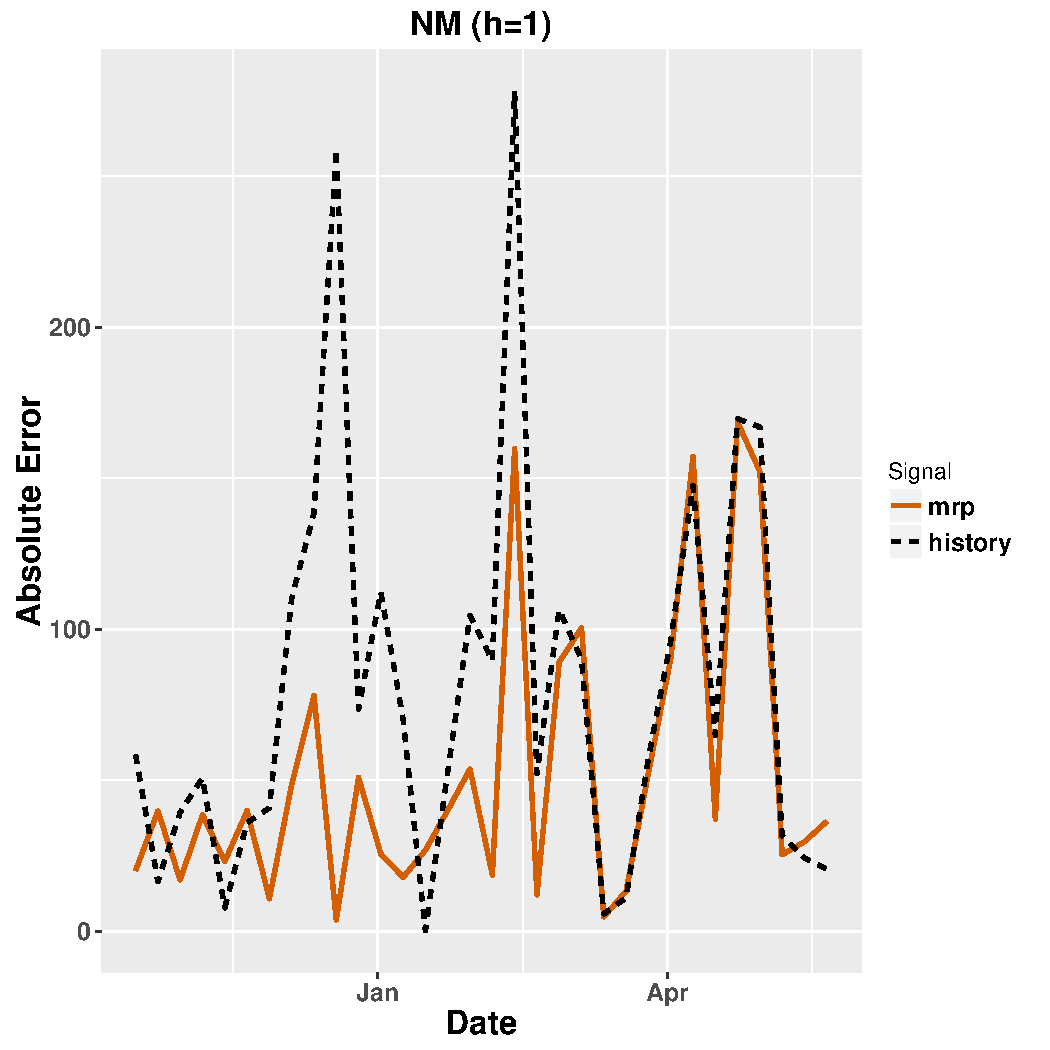
\includegraphics[width=.45\linewidth]{NM_h_1_Abs_error}&
  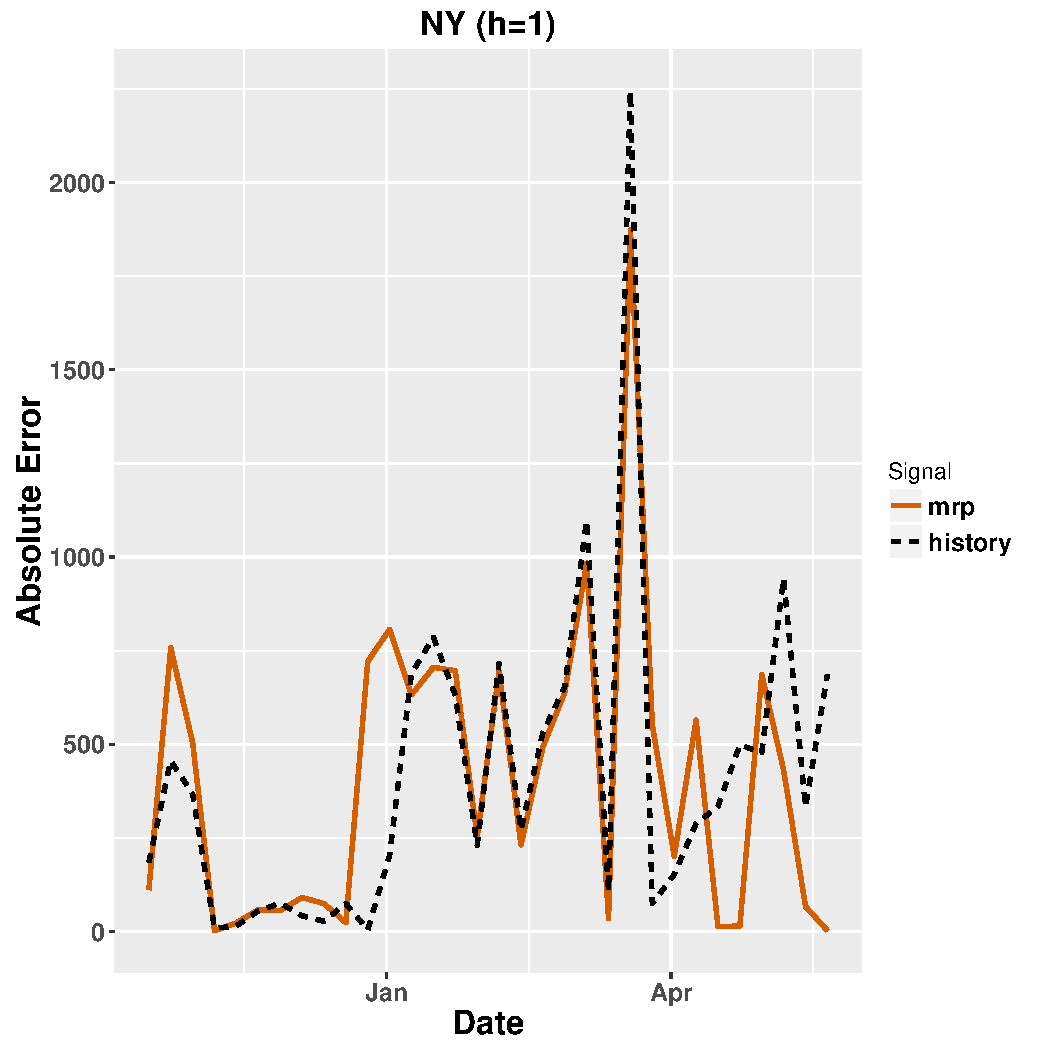
\includegraphics[width=.45\linewidth]{NY_h_1_Abs_error}\\
    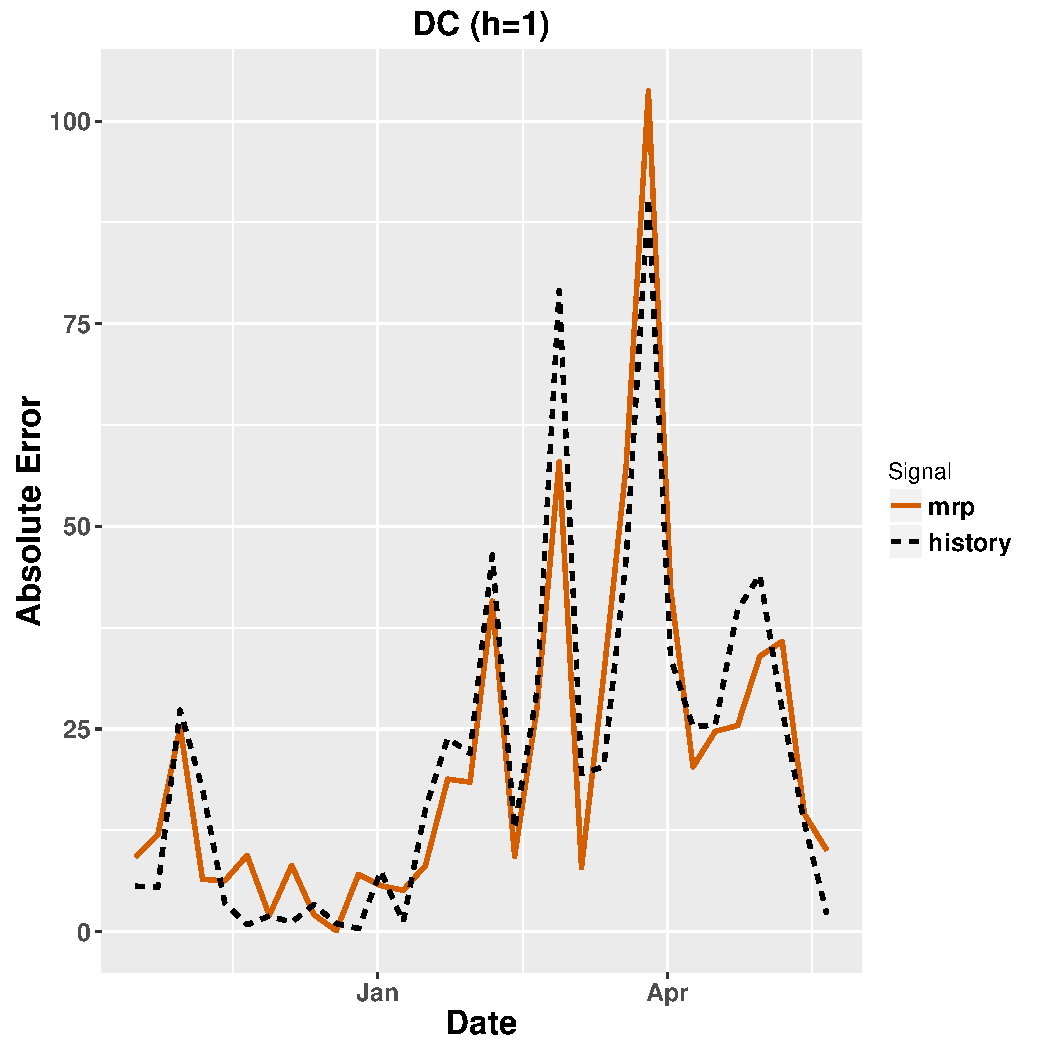
\includegraphics[width=.45\linewidth]{DC_h_1_Abs_error}&
        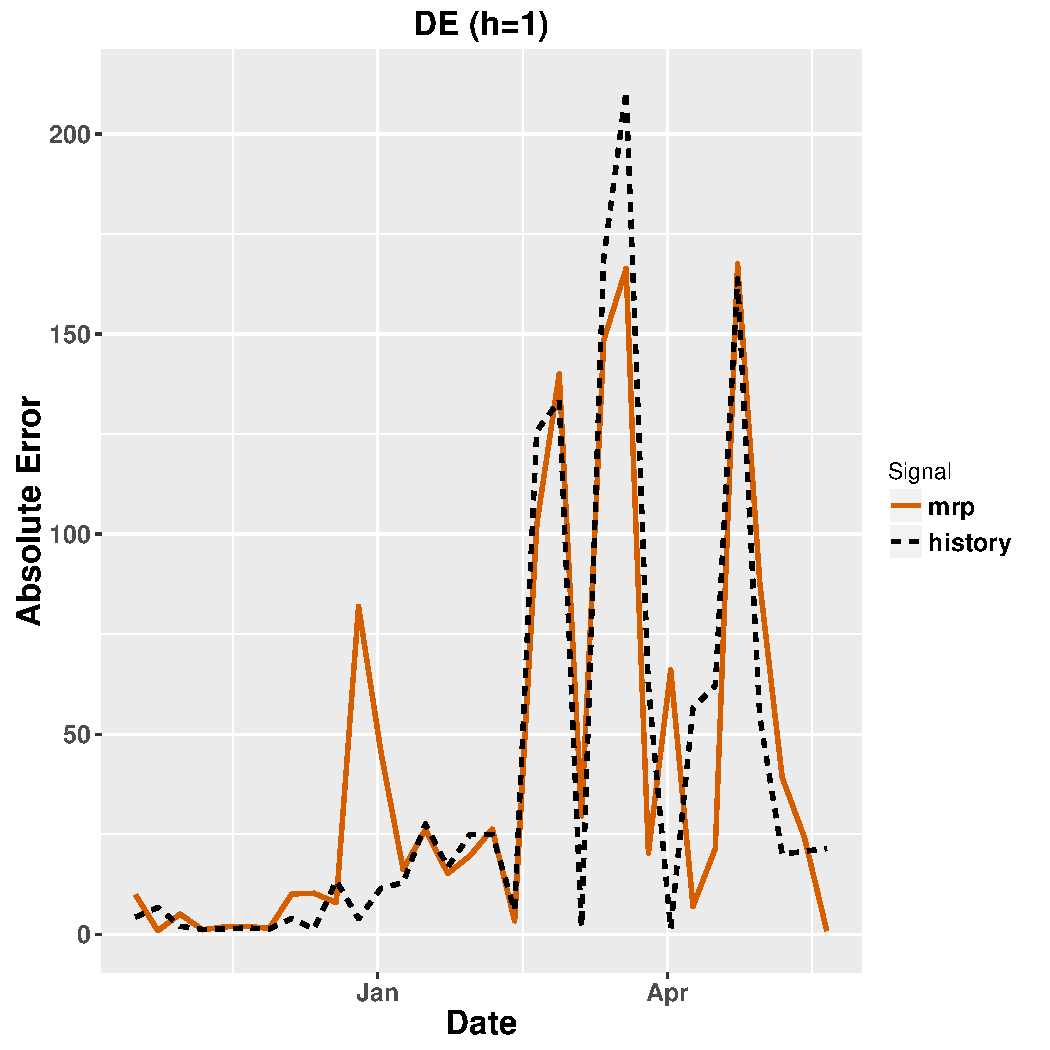
\includegraphics[width=.45\linewidth]{DE_h_1_Abs_error}
 \caption{a) h=1 indicates week ahead absolute errors for history against the MRP signal for NM,  NY, DC and DE.}
  \label{fig:State_Abs_Errs}
\end{figure}

Figure \ref{fig:State_Abs_Errs} shows that incorporating the MRP signal in the SARIMA-X model controls the variance in the prediction error (the absolute errors are less spiky) . These plots visually represent what is presented in Table 3 in the state level RMSE results. As a general approach for predicting time dependent metrics, the inclusion of appropriate exogenous signals such as the MRP signal can have a considerable beneficial impact on the prediction quality.

%\subsection{Results and Forecast Analysis}

%Table \ref{tab:h1results} reveals that improvement over the historical model forecasts especially for the $2$-week ahead errors. This makes sense since relying only on the historical signal as a predictor for $h=2$ introduces more uncertainty due to the additive nature of forecast errors and using predictive exogenous signals can partially reduce this uncertainty. In particular, depending on the predictive power of the exogenous signals the forecast error spread (or uncertainty) can be controlled leading to relatively more stable forecasts. This is especially useful if the historical signal is more volatile, as is the case with the states. This can also be seen in the box plot (Figure \ref{fig:CA_DE_Box}) of the absolute forecast errors on the held out period for CA and DE.

% \subsection{CDC Regions}

% We also applied our methodology to the CDC regions. The ILI-rates for the CDC region are extremely smooth and stable in general and as also pointed out in \citet{lazer_etal_2014} historical signals are very powerful predictors. For completeness we show $2$-step ahead rolling prediction errors using model \eqref{eq:SAR-Model} for all the CDC regions. For the $1$-step ahead errors results with and without are very similar and are therefore omitted.

% \begin{figure}[!htbp]
% \begin{centering}
% \begin{tabular}{ccc}
%    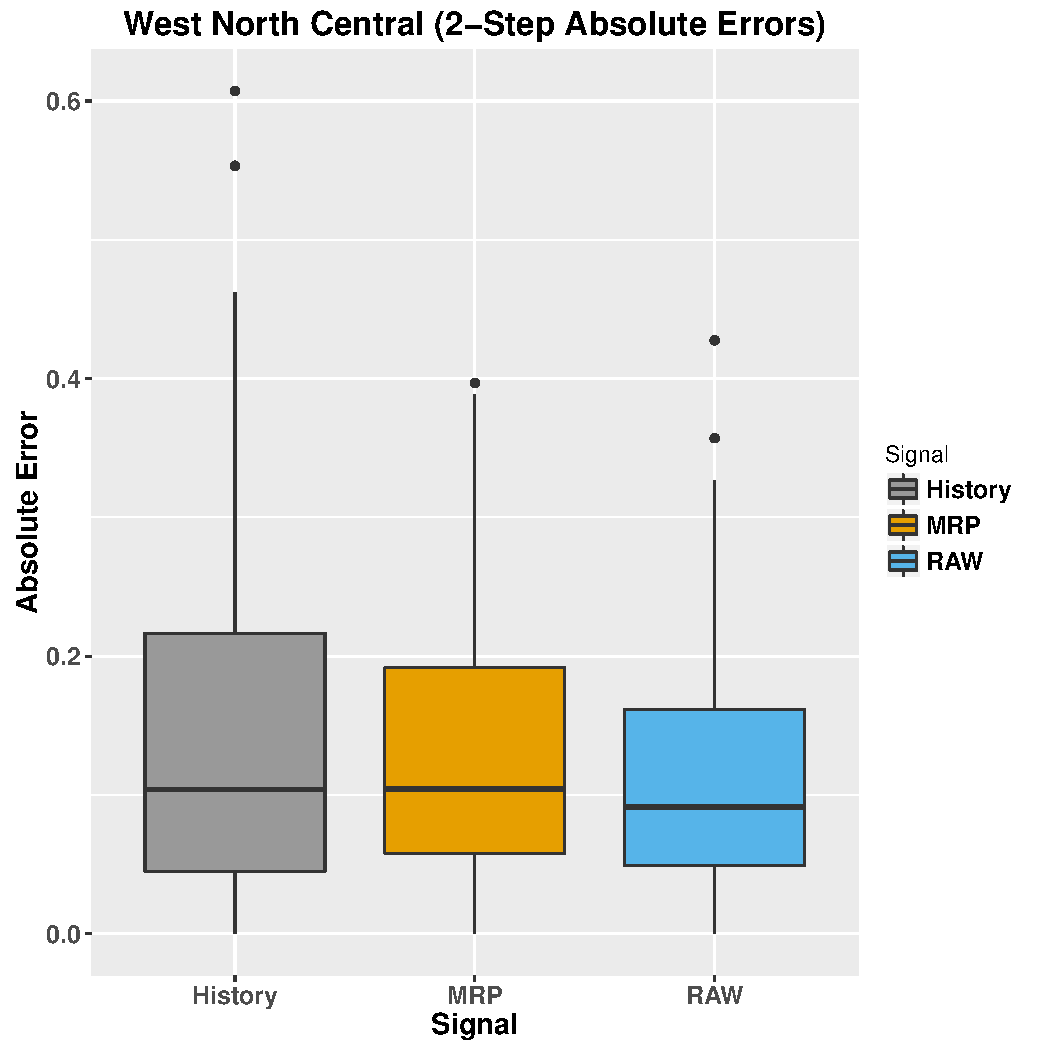
\includegraphics[width=.5\textwidth]{WNCBox_h_2.pdf}&
%    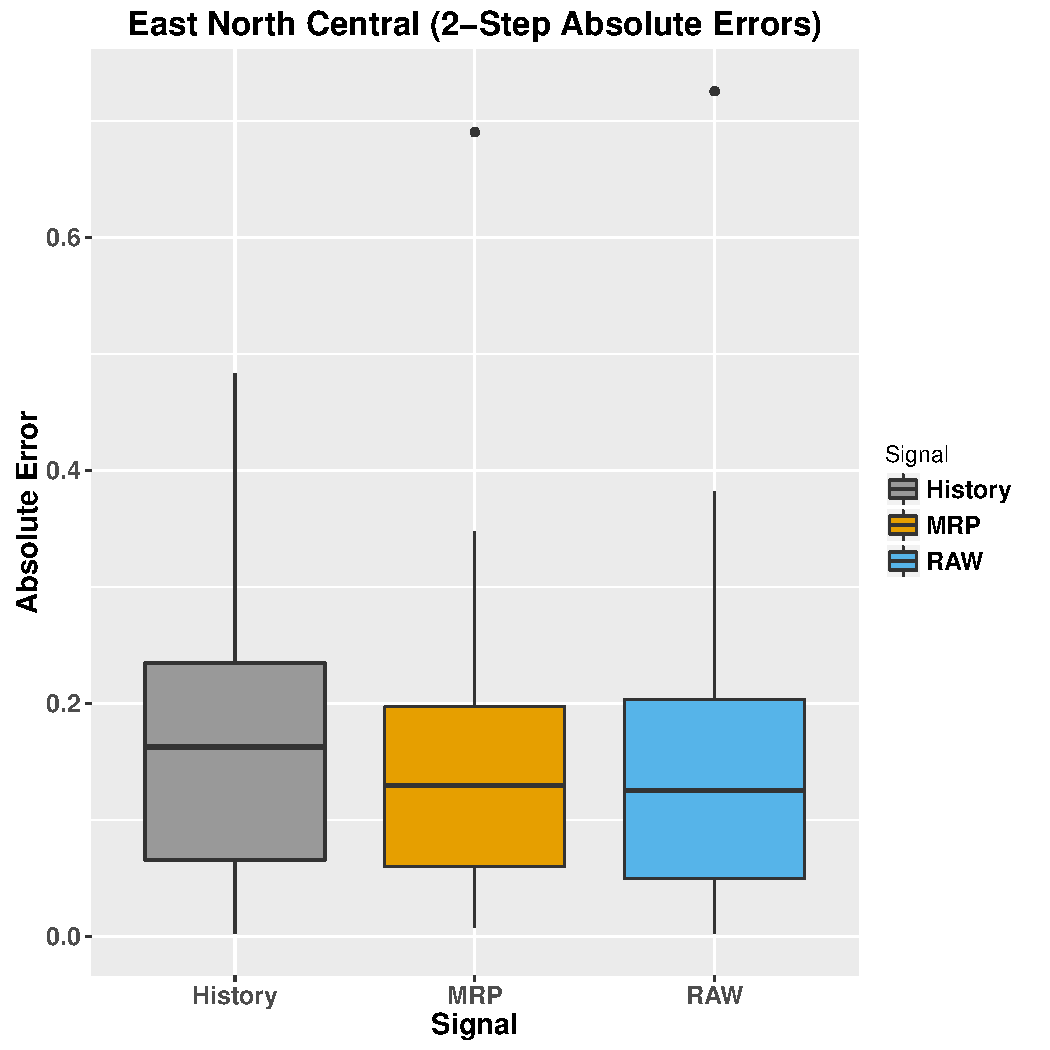
\includegraphics[width=.5\textwidth]{ENCBox_h_2.pdf}&
%   \end{tabular}
% \end{centering}
%   \caption{Absolute forecast errors Box plot of West and East North Central CDC regions (h=2). }
%     \label{fig:WNC_ENC_Box}
% \end{figure}

% Table \ref{tab:cdcMSE} reveals that in almost all the cases the inclusion of our exogenous signals boosts accuracy with significant improvement in West North Central, West South Central and East North Central in particular. The box plots for the absolute forecast errors reveal a decrease in the spread as also observed in the State level forecasts.




%Additionally we observe that using combinations of signals often improves the prediction accuracy. The smoothed and re-weighted signal reduces the impact of particularly active regions of states where more web searches are generated. It removes inferred demographic biases in search behavior. However, our results suggest that these active regions are providing at least some additional information about changes in flu prevalence, improving the fit of the model over a smoothed and re-weighted signal alone. As a consequence, combinations of raw and smoothed/re-weighted signals are frequently the most powerfully predictive model specification.

% Please add the following required packages to your document preamble:
% \usepackage[table,xcdraw]{xcolor}
% If you use beamer only pass "xcolor=table" option, i.e. \documentclass[xcolor=table]{beamer}
% \begin{figure}[!htbp]
% \begin{centering}
% \begin{tabular}{ccc}
%    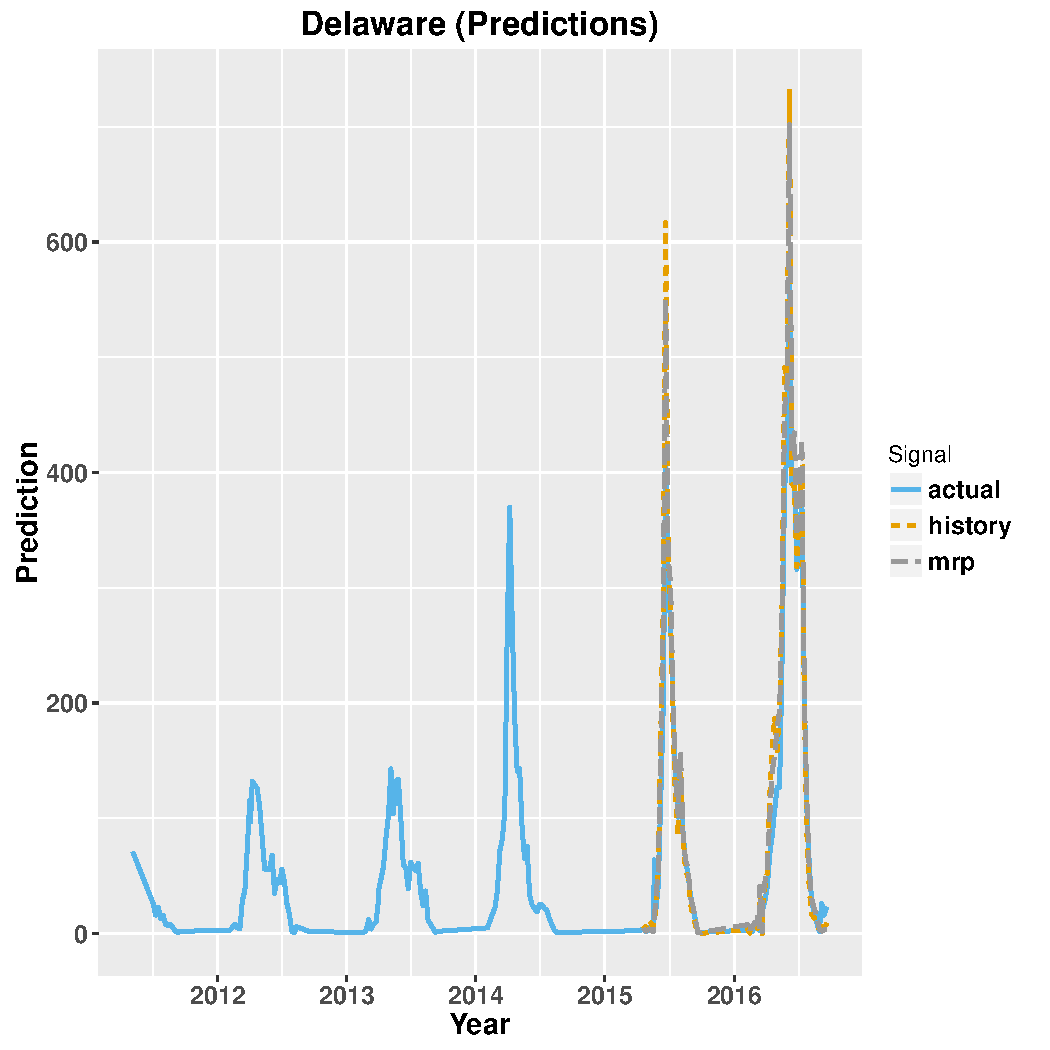
\includegraphics[width=.5\textwidth]{DE_h_1.pdf}&
%    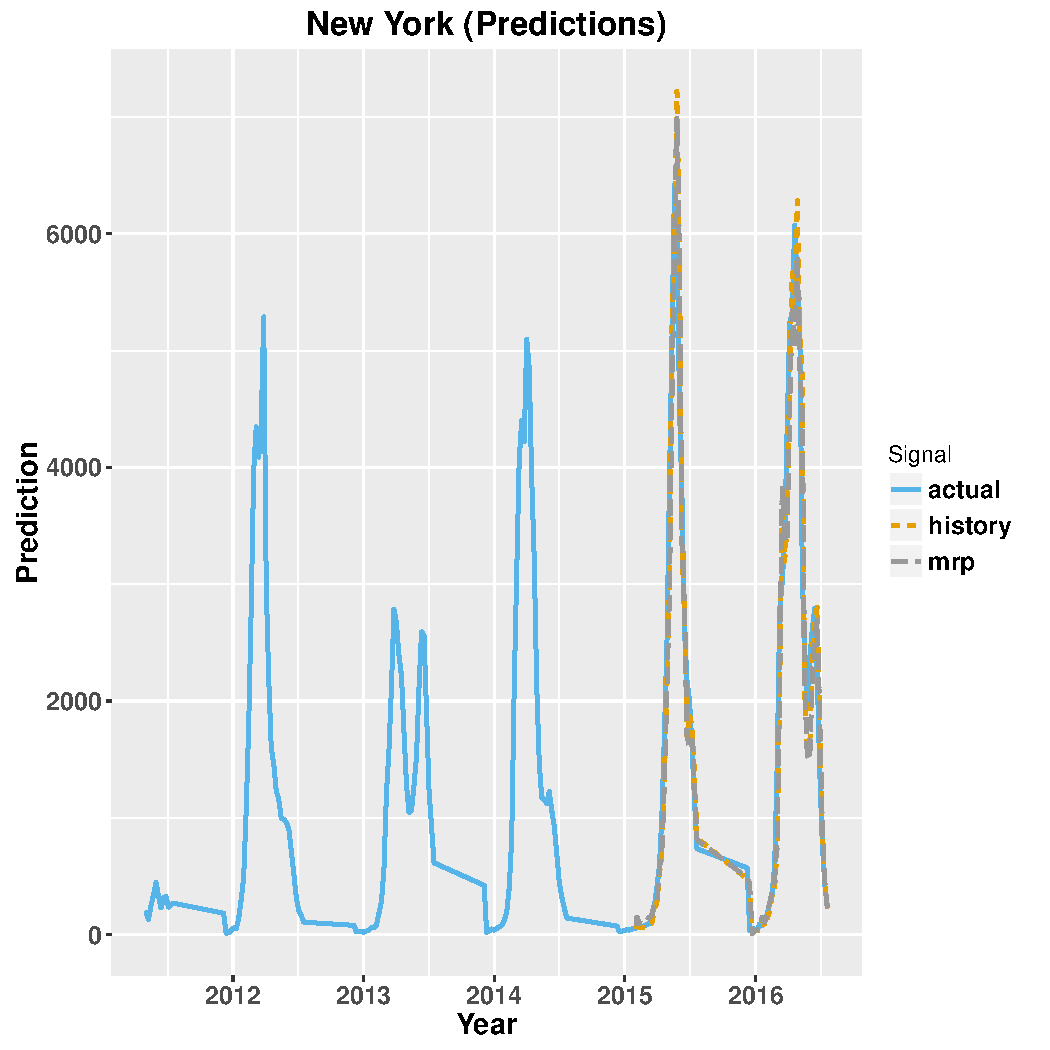
\includegraphics[width=.5\textwidth]{NY_h_1.pdf}&
%   \end{tabular}
% \end{centering}
%   \caption{Predictions for Delaware and New York for $h=1$. MRP predictions do not overestimate the peaks compared to the historical model.}
%   \label{fig:DE_NY_Preds}
% \end{figure}


% Please add the following required packages to your document preamble:
% \usepackage[table,xcdraw]{xcolor}
% If you use beamer only pass "xcolor=table" option, i.e. \documentclass[xcolor=table]{beamer}

% \subsection{Qualitative Analysis and Discussion}

% Supporting our claims in the previous section Figure \ref{fig:DE_NY_Preds} reveals that incorporating the MRP signal in the SARIMA-X model prevents the prediction from overshooting. The historical model anticipates a bigger peak while this is not reflected in the MRP signal included model predictions. Thus, as a general approach for predicting time dependent metrics, the inclusion of appropriate exogenous signals can have a considerable beneficial impact on the prediction quality.

% In some cases we find that the MRP smoothed estimates do not outperform the raw  estimates from our survey-based textual methods. The reason for this, we suspect, is that some examples come from 1) demographically homogeneous areas of the country where the distribution of flu search prevalence tends to be more uniform and/or 2) the samples provided at a given period of time and place are, by chance, sufficiently representative of the underlying distribution of flu search prevalence. In both cases, we suspect that the MRP simply smooths out the distribution too much.

% In addition, when the MRP improves over the Raw, we can see the Raw does more poorly even than history (examples Mountain, New England, South Atlantic). However, when the MRP does worse than the Raw, the MRP still does better than history, suggesting that the MRP performs consistently better than history.

%\section{Limitations}


%In this paper, we tackle a subset of the problems of ILI prediction in the context of search query data. We offer two primary advances. First, we use survey data and human-machine ensembles to select positive predictors of flu experiences. Next, we leverage these insights and integrate demographic data to account for the uneven propensity of flu search. We use these data to model the social and demographic drivers of flu searches. Our method forecasts ILI prevalence at the national and state levels using demographically smoothed (noise-reduced) and re-weighted (bias-reduced) estimates of flu-like query volumes. This approach has potentially wide applicability to problems of forecasting time series of small to medium length using search query or social media data.

%We test our model on state-level ILI rates from 4 states and national CDC rates. Our model substantially improves fit over history alone, and yields similar improvements across the US as a whole, states, and flu seasons. Our results suggest that a combination of demographically re-weighted search signals and human-aided query labeling produces an accurate and near real-time model of flu prevalence at the state level. The evidence suggests that by constructing a model which takes into account demographics and social factors of search behavior, we can improve over raw search volumes and flu history alone. This provides important lessons for query and social media-based flu tracking systems.

\singlespace
\bibliography{flu_citations}
\bibliographystyle{apsr}


\end{document}
